% !TeX root = ../../main.tex
% Add the above to each chapter to make compiling the PDF easier in some editors.

\chapter{Benchmark Evaluation}\label{ord:ch5}

All user interactions were recorded during their participation in the benchmark. 
In this chapter, we evaluate this acquired data.
To judge if the differences of methods are significant statistical methods are applied, which are in general supported by the large amount of data with \getNumberBenchmarkAnnotations annotations from \getNumberBenchmarkRuns runs on the benchmark study.
To illustrate how annotations from the benchmark study look like Figure \ref{fig:ch5:segmentation_examples} provides few exemplary annotations, while a detailed insight of 27 predictions from the methods watershed, \gls{dextr} and \gls{iog} is given in Figure \ref{fig:appendix_model_predictions}.

%TODO Bitte die gesamte Arbeit nochmal durchlesen und auf Plural vs. Singular bei den Verben und den Substantiven achten! Solche Fehler reduzieren die Lesbarkeit und schmälern die schönen Ergebnisse!
%TODO beispielhafte grafic that shows annotations
\begin{figure} [b]
	\centering
	\begin{subfigure}[t]{0.3\textwidth}
		\centering
		
\includegraphics[width=\textwidth]{figures/placeholder.png}
		\caption{
			tbd
		}
	\end{subfigure}
	\hfill
	\begin{subfigure}[t]{0.3\textwidth}
		\centering
		
\includegraphics[width=\textwidth]{figures/placeholder.png}
		\caption{
			tbd
		}
	\end{subfigure}
	\hfill
	\begin{subfigure}[t]{0.3\textwidth}
		\centering
		
\includegraphics[width=\textwidth]{figures/placeholder.png}
		\caption{
			tbd
		}
	\end{subfigure}
	\caption[tbd]{
		tbd
	} \label{fig:ch5:segmentation_examples}
\end{figure}


% !TeX root = ../../main.tex
% Add the above to each chapter to make compiling the PDF easier in some editors.

\section{Improvement In Time And IoU}\label{ord:ch5:sec1}

This section focuses on the annotation time $time_{annot}$ and the precision measure $IoU$ from the benchmark measurements.
First, the relationship between time and user clicks is examined.
Second, the $IoU$ is evaluated based on the four benchmark methods.
Third, the same evaluation evaluation is performed with the $time_{annot}$. 


\subsection{Correlation Between Time And Clicks}\label{ord:ch5:sec1:subsec1}

% RE-1464 
In the following the relationship between time and the user interaction as clicks and strokes is investigated, in order to promote the further analysis, which is strongly based on $time_{annot}$. 
As introduced in Subsection \ref{ch2:sec3:eval_interactive_methods}, a common metric to measure the level of user interaction is the number of clicks $n_{clicks}$.
Thereby, $n_{clicks}$ functions as indicator for $time_{annot}$, which is the more meaningful variable in terms of ranking the amount of user interaction.
In general, $n_{clicks}$ is not necessarily fair indicator, because the time per click may differ for user interaction of methods with varying complexity.

In the benchmark study the user interaction was recorded by the number of clicks $n_{clicks}$, number of strokes $n_{strokes}$, and required time to perform the strokes $time_{strokes}$ .
The informative value of each single variable is limited, because the user interaction may consists out of either only clicks or strokes, or a combination of both.
The stroke related variables are combined to the weighted strokes $ ws $ by
\begin{equation} \label{equ:ws}
	ws = f_{stroke} \cdot time_{strokes} + n_{strokes} 
\end{equation}
with the weighting factor $ f_{stroke} $.
Based on a manual analysis of the data $ f_{stroke} = 1.0 $ was determined, so that one second of stroking has the same value as one click, which is expected to be a fair trade-off between clicks and strokes.
To facilitate the comparison a single variable $ cws $ is established by 
\begin{equation}
	cws = n_{clicks} + ws
\end{equation}
which combines clicks and strokes.

The relationship of the single variables is presented within a correlation matrix in Table \ref{tab:ch5:correlation-matrix}.
The reliability of the correlation matrix is supported by the size of the dataset with \getNumberBenchmarkAnnotations annotations.
This includes the annotations from all four benchmark methods, between which no distinction is made in this subsection.
% Correlation between time_{annot} and cws
The correlation between the time and weighted clicks and strokes $ corr \left(time_{annot}, cws \right) = 0.8610 $ is strong.
This confirms the relationship between these variables and supports their suitability for further evaluation.

Although, it should be noted that, the correlation value of $ time_{annot} $ and $ cws $ is not maximal.
This assists the hypothesis that $ cws $ does not constitute a flawless representation of $ time_{annot} $ and thereby is not a perfectly suitable performance measure.
However, $ cws $ is still sufficient for the comparison of interactive methods, but the limitations have to be noted.
For the further evaluation mostly $ time_{annot} $ will be used to represent the user interaction.

Last, attention should be drawn to the correlation between \gls{iou} and time \linebreak $ corr \left(time_{annot}, IoU \right) = 0.0379 $.
So in general, a long annotation time does not necessarily correspond to a high \gls{iou}.
This indicates, that some methods can achieve a good IoU in little time, while other methods require more time.
The annotation time is evaluated in detail in Subsection \ref{ord:ch5:sec1:subsec3}. 

\begin{table}[h!]
	\centering
	\resizebox{\textwidth}{!}{
	\begin{tabular}{l|c c c c c c c}
		\toprule 		
							& $ time_{annot} $ 	
										& $ n_{clicks} $ 	
													& $ n_{strokes} $ 
																& $ time_{strokes} $ 
																			& $ ws $ 	& $ cws $   & $ IoU $ \\
		\midrule
		$ time_{annot} $	& 1 		& - 		&  -		& - 		& - 		& - 		& - \\ 
		$ n_{clicks} $		& 0.7085	& 1 		&  - 		& - 		& - 		& - 		& - \\ 
		$ n_{strokes} $ 	& 0.7391 	& 0.6169 	&  1 		& -		   	& - 		& - 		& - \\ 	
		$ time_{strokes} $ 	& 0.7069 	& 0.3309	&  0.7949	&  1 		& - 		& - 		& - \\ 
		$ ws $				& 0.7500 	& 0.4376 	&  0.8973	&  0.9811 	&  1 		& - 		& - \\ 
		$ cws $		  		& 0.8610 	& 0.8261	&  0.9028	&  0.7976 	&  0.8682 	& 1 		& - \\ 
		$ IoU $    			& 0.0379 	& 0.0455	&  0.0004	& -0.0101 	& -0.0073 	& 0.0206 	& 1 \\ 								
		\bottomrule
	\end{tabular}}
	\caption[Correlation table]{
		Correlation table based on the \textit{Pearson} standard correlation coefficient \cite{Kirch08-CorrPearson}.
		The redundant part of the table is left empty. 
		The variables $ n_{clicks} $, $ n_{strokes} $, $ time_{strokes} $, and $ ws $ all show a intermediate correlation with $ time_{annot} $, while their combination $ cws $ shows a strong correlation with $ 0.8610 $. 
		The correlation between $ IoU $ and $ time_{annot} $ indicates almost no relationship $ 0.0379 $.
	}\label{tab:ch5:correlation-matrix}
\end{table}


\subsection{Analysis Of IoU}\label{ord:ch5:sec1:subsec2}

In the following the $IoU$ is evaluated in detail by the application of the statistical methods introduced in Section \ref{ord:ch2:sec4}, but first a limitation of the benchmark study is set forth.

% Limitation - The resulting mask was shown to the user, which may lead to futher editing resulting in a better IoU and more time
It may be problematic, that the design of the user interaction differs between the benchmark methods.
For the \gls{dextr} and \gls{iog} method the user interaction is strictly guided due to the limited amount of clicks for the initial prediction.
For the polygon and watershed method the user interaction is designed more open and therefore, gives the user more freedom of choice.
With the open design of these methods, the user may feel that he has not applied them well enough, if the shown results are unsatisfactory.
As a results, the user may directly further edit the initial annotation in order to improve it.
In contrast the strong guidance for the \gls{dextr} and \gls{iog} method gives the user confidence in having used the method correctly and assigns an insufficient annotation to the method itself.
In general, users may find it more difficult to accept bad annotations, if the method gave them a lot of freedom in creating it. 
This assumption also applies in reverse, for easy acceptance by methods with strong guidance.
Therefore, the annotations may have a similar \gls{iou}, but the time spent differs as shown in Subsection \ref{ord:ch2:sec1:subsec3}.
If the annotations had to be created in a certain time, the \gls{iou} would also be different, but it was decided against such a setup.


\subsubsection{Data Transformation}
Subsection \ref{ord:ch2:sec4:subsec1} already introduced the normality assumption for statistical methods as the Student's t-test and suggests a transformation of the data.
The histogram of the $IoU$ illustrates that the sample is not distributed normally as shown in Figure \ref{fig:ch5:sec1:data_raw}.
The data points are heavily skewed to the right. 
This is caused by many data points with a high \gls{iou} and comparatively few with a low \gls{iou}, produced by general good segmentation results.

In order to normalize the raw sample $ X_{raw} $, \cite{PS16-Statistics} suggests the logarithmic function
\begin{equation} \label{equ:trans_iou}
	X_{trans} = \frac{1}{2} \cdot \log \left( \frac{1 + X_{raw}}{1 - X_{raw}}\right) 
\end{equation}
to transform $ X_{raw} $ into $ X_{trans} $.
In Figure \ref{fig:ch5:sec1:data_transformed}, $ X_{trans} $ demonstrates the characteristics of a normal distribution.
Further the normality of $ X_{trans} $ is demonstrated by the probability plot shown in Figure \ref{fig:ch5:sec1:probplot}.

\begin{figure} [h]
	\centering
	\begin{subfigure}[t]{0.3\textwidth}
		\centering
		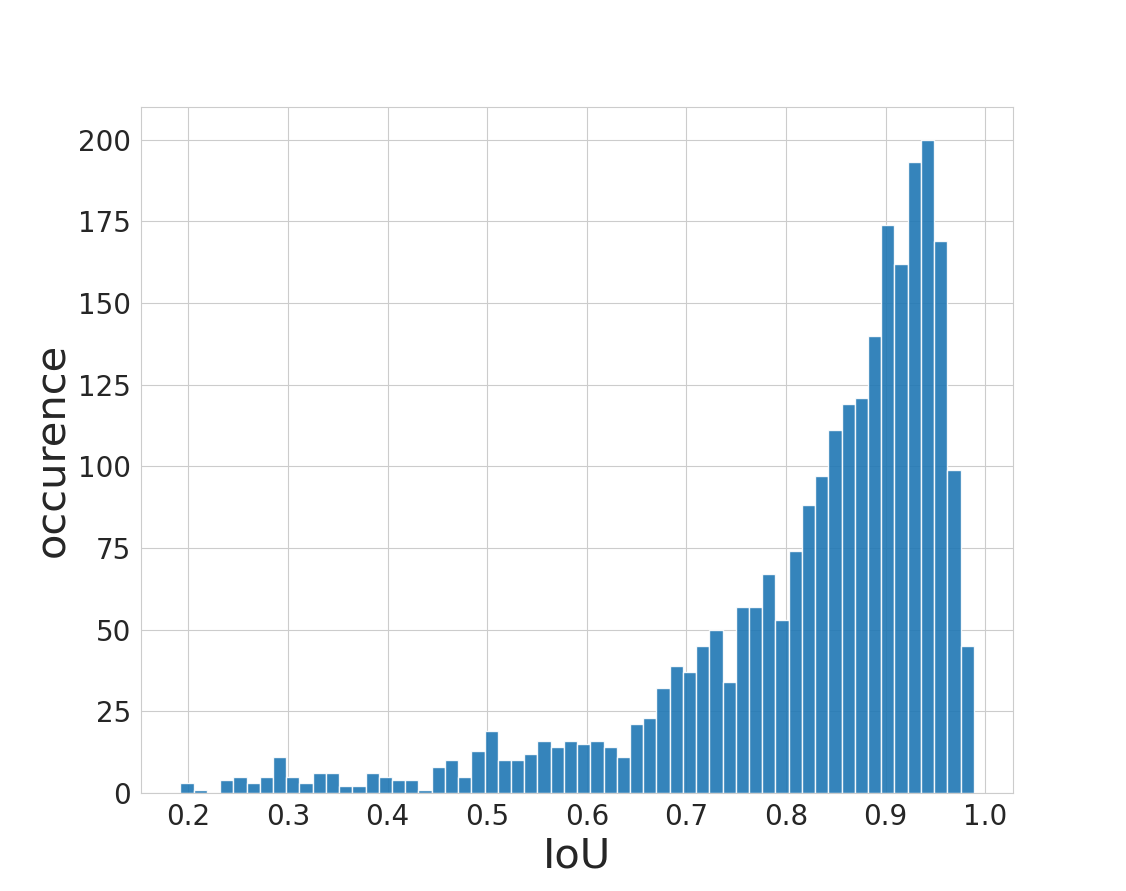
\includegraphics[width=\textwidth]{figures/chap51_iou_raw.png}
		\caption{
			Histogram of the $ IoU $ values as raw and unprocessed sample $ X_{raw} $.
		}\label{fig:ch5:sec1:data_raw}
	\end{subfigure}
	\hfill
	\begin{subfigure}[t]{0.3\textwidth}
		\centering
		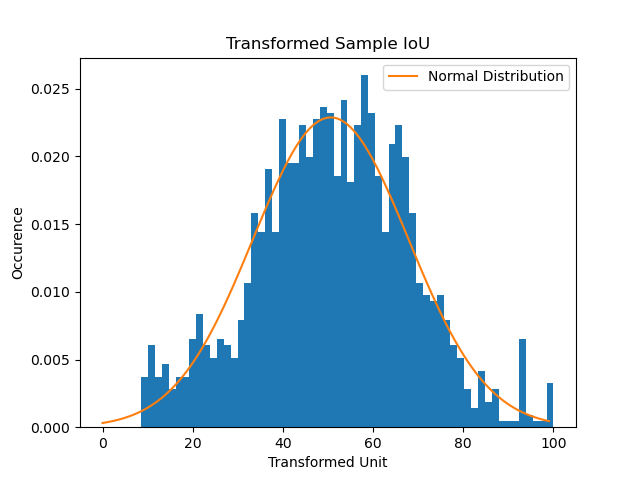
\includegraphics[width=\textwidth]{figures/chap51_iou_trans.png}
		\caption{
			Histogram of the transformed sample $ X_{trans} $ with a fitted normal distribution.
		} \label{fig:ch5:sec1:data_transformed}
	\end{subfigure}
	\hfill
	\begin{subfigure}[t]{0.3\textwidth}
		\centering
		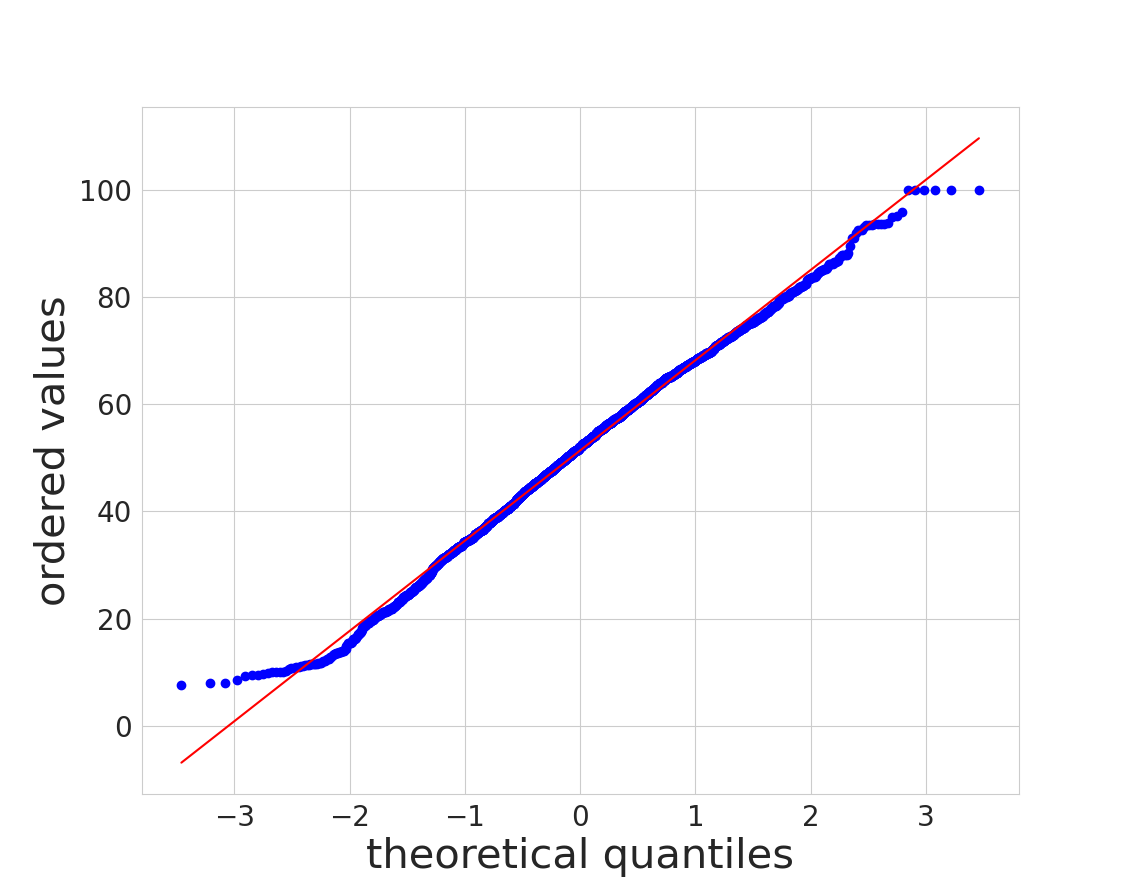
\includegraphics[width=\textwidth]{figures/chap51_iou_probplot.png}
		\caption{
			Normal probability plot of $ X_{trans} $.
		}\label{fig:ch5:sec1:probplot}
	\end{subfigure}
	\caption[Sample Transformation $ IoU $]{		
		The sample $ X $ is transformed to achieve a normal distribution.
		As shown in a) $ X_{raw} $ is skewed to the right and not distributed normally.
		The transformation was performed by Equation \ref{equ:trans_iou}.
		The result of the transformation is $ X_{trans} $ and features normal characteristics, as illustrated in b) by the curve of the fitted normal distribution.
		In c) a normal probability plot confirms the normality in $ X_{trans} $.
	}\label{fig:ch5:sec1:data_transformation_iou}
\end{figure}


% Hypothesis testing
\subsubsection{Hypothesis Testing}

In the following multiple hypothesis tests are described, which divide the sample in two and four factors.

First, it is tested if \gls{dl} based methods (\gls{iog} and \gls{dextr}) are advantageous over classical methods (polygon and watershed).
This more general test results in the two factors $ IoU_{classical} $ and $ IoU_{dl} $.
Three different hypothesis tests are applied on these two factors.
Student's t-test evaluates the mean of the factors, Kruskal-Wallis the median of the factors, and Mann-Whitney the general tendency of the factors as introduced in Subsection \ref{ord:ch2:sec4}.
The detailed settings and results of the tests are presented in Table \ref{tab:ch5:tests_on_iou}.
All three tests come to the conclusion to accept $ H_{0} $, that in general the $ IoU $ of \gls{dl} based methods do not differ significantly from the $ IoU $ of classical methods.
The information value of this conclusion is especially strong, due to the application of three different tests with various null hypotheses.

\begin{table}[h!]
	\centering
	\resizebox{\textwidth}{!}{
	\begin{tabular}{l|c c c}
		\toprule 		
			 			& Student's t-test	& Kruskal-Wallis test 	& Mann-Whitney U-test \\
		\midrule
		data			& $ X_{trans} $		& $ X_{raw} $ 	 		& $ X_{raw} $ 	\\ 
		$H_{0}$			& $ \overline{IoU}_{classical} = \overline{IoU}_{dl} $ 
											& $ med \left( IoU_{classical} \right)  = med \left( IoU_{dl} \right) $ 
																	& $ ten \left( IoU_{dl} \right)  = ten \left( IoU_{classical} \right) $ 	\\
		$ H_{A} $		& $ \overline{IoU}_{classical} < \overline{IoU}_{dl} $ 
											& $ med \left( IoU_{classical} \right) < med \left( IoU_{dl} \right) $ 
																	& $ ten \left( IoU_{dl} \right) \not= ten \left( IoU_{classical} \right) $ 	\\
		$ \alpha $		& $ 5\% $ 			& $ 5\% $ 		 		& $ 5\% $ 		\\ 	
		Statistic		& 0.3494			& 825786	     		& 0.0035    	\\ 
		$ \textnormal{\textit{p-value}} $ 
						& 0.7268 			& 0.4765 		 		& 0.9529		\\ 
		$ H_{0} $		& accepted 			& accepted		 		& accepted 		\\
		\bottomrule
	\end{tabular}}
	\caption[Hypothesis Tests on $ IoU $]{
		Overview and results of the statistical tests.
		The $ IoU $ is evaluated by various values as the mean, median and tendency of the sample.
		Both factors $ IoU_{classical} $ and $ IoU_{dl} $ contain 1286 annotations.
		If the $ \textnormal{\textit{p-value}} $ is greater than the significance level $ \alpha $, $ H_{0} $ is accepted.
		The same result is achieved by all three different statistical tests, which supports its reliability.
	}\label{tab:ch5:tests_on_iou}	
\end{table}

% Kruskal-Wallis Test for four factors rejects H0.
Second, the $ IoU $ is evaluated in detail, thereby the Kruskal-Wallis test is applied using the four benchmark methods as factors.
The corresponding null hypothesis 
\begin{equation}
	H_{0}: med \left( IoU_{Polygon} \right) = med \left( IoU_{Watershed} \right) = med \left( IoU_{IOG} \right) = med \left( IoU_{DEXTR} \right)
\end{equation}
states, that the median values do not differ significantly.
$ H_{A} $ assumes that $ H_{0} $ is not true, but does not define which factor is different.
As result the statistic returns $ \textnormal{\textit{p-value}} = 7.8 \cdot 10 ^{-8} $, therefore $ H_{0} $ is rejected and $ H_{A} $ accepted at $ \alpha=5\% $.

It can be determined what factors differ significantly, by the application of the DSCFs  test \cite{CF91-dscf}.
In this test it is shown that, $ med \left( IoU_{DEXTR} \right) $ is greater, while $ med \left( IoU_{IOG} \right) $ is lower than the other factors. 
This is also visualized in Figure \ref{fig:ch5:sec1:iou_box_plot} and may seem like a small difference, but the statistical relevance is confirmed.
Conspicuous in the plot shown are the high amount of outliers and the wide range of the lower quarter of the box plot.
An explanation for this are demanding annotations from the domain $ anomaly $ or the failure of the methods on single annotations.
The number of outliers may seem large, but must be put in proportion to the size of the data with \getNumberBenchmarkAnnotations annotations.

\begin{figure}
	\centering
	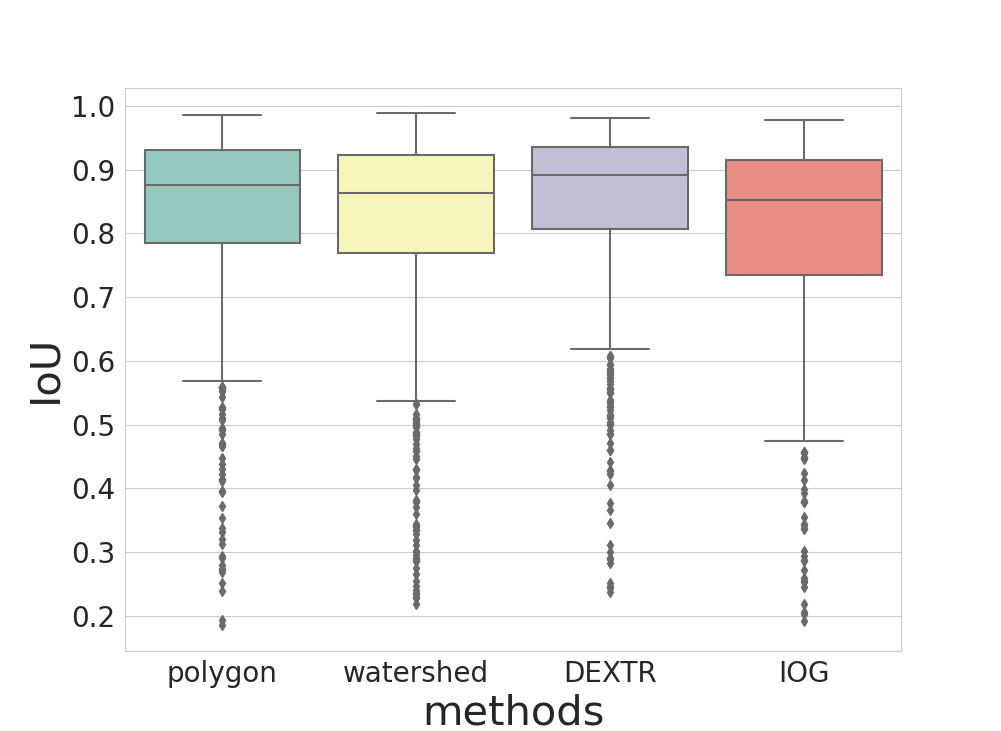
\includegraphics[width=0.6\textwidth]{figures/chap51_iou_boxplot.png}
	\caption[Box plots method on $ IoU $]{
		Box plot of the $ IoU $ for the four benchmark methods.
		$ med \left( IoU_{DEXTR} \right) $ is slightly greater than the other factors, while $ med \left( IoU_{IOG} \right) $ is the smallest worst.
		The classical methods to not differ significantly in their median values $ med \left( IoU_{Polygon} \right) $ and $ med \left( IoU_{Polygon} \right) $.
	} \label{fig:ch5:sec1:iou_box_plot}
\end{figure}



\subsection{Analysis Of Time}\label{ord:ch5:sec1:subsec3}
% RE-1466
Now the $time_{annot}$ is evaluated, the evaluation procedure is analog to the previous evaluation of the $IoU$.
\subsubsection{Data Transformation}

The histogram of the raw sample for the $time_{annot}$ does not fit a normal distribution as shown in Figure \ref{fig:ch5:sec1:time_raw}.
Instead, the data points are heavily skewed to the left, because $time_{annot}$ is usually short, but can also be larger.
\cite{PS16-Statistics} suggests to transform the sample by the logarithmic function 
\begin{equation} \label{equ:trans_time}
	X_{trans} = \log \left( X_{raw} \right) 
\end{equation}
to adapt the shape of a normal distribution, $X_{trans}$ is shown in Figure \ref{fig:ch5:sec1:time_transformed}.
$X_{trans}$ is similar to a normal distribution, which is also supported by the corresponding normal probability plot illustrated in Figure \ref{fig:ch5:sec1:time_probplot}

\begin{figure} [h]
	\centering
	\begin{subfigure}[t]{0.3\textwidth}
		\centering
		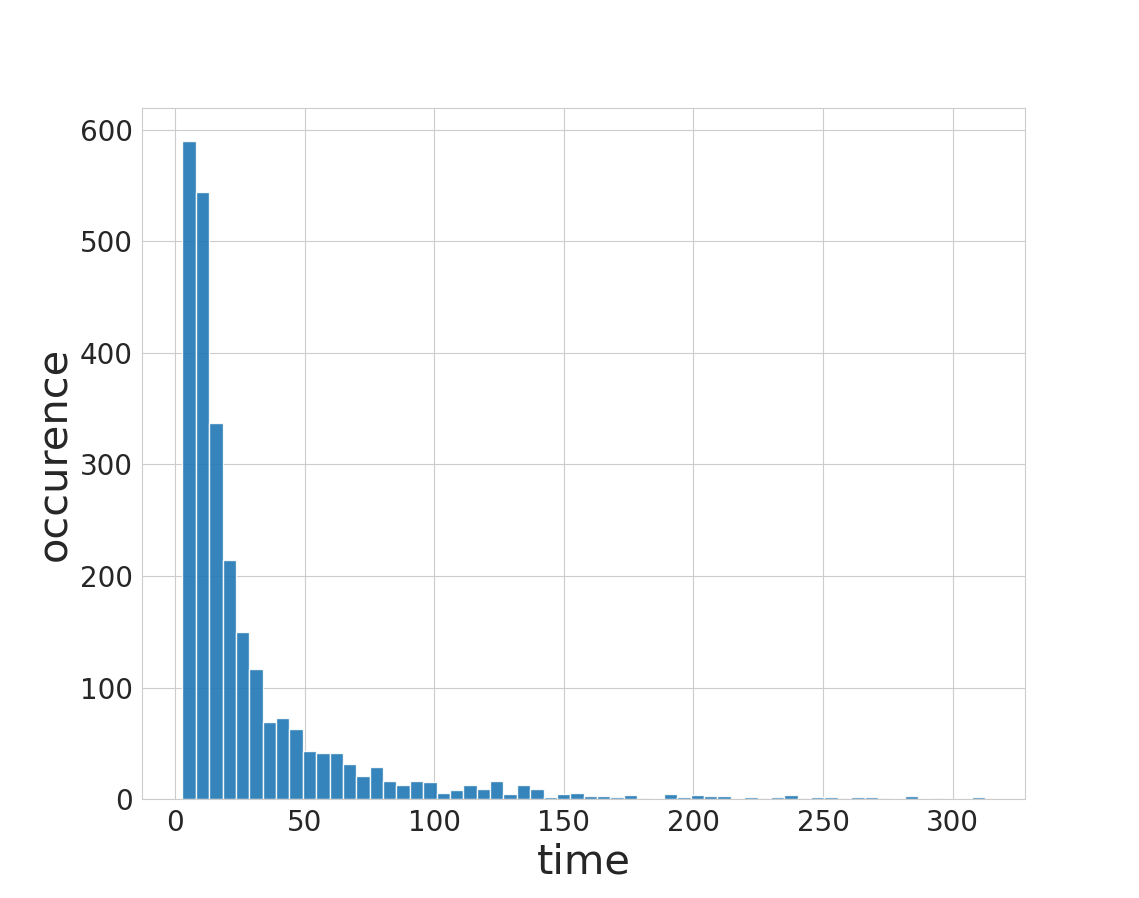
\includegraphics[width=\textwidth]{figures/chap51_time_raw.png}
		\caption{
			$ time_{Annot} $ as raw and unprocessed sample $ X_{raw} $.
		}\label{fig:ch5:sec1:time_raw}
	\end{subfigure}
	\hfill
	\begin{subfigure}[t]{0.3\textwidth}
		\centering
		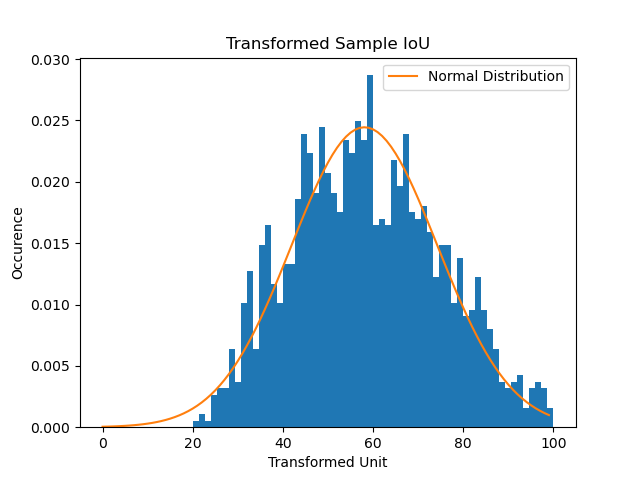
\includegraphics[width=\textwidth]{figures/chap51_time_trans.png}
		\caption{
			Transformed sample $X_{trans}$ with fitted normal distribution.
		} \label{fig:ch5:sec1:time_transformed}
	\end{subfigure}
	\hfill
	\begin{subfigure}[t]{0.3\textwidth}
		\centering
		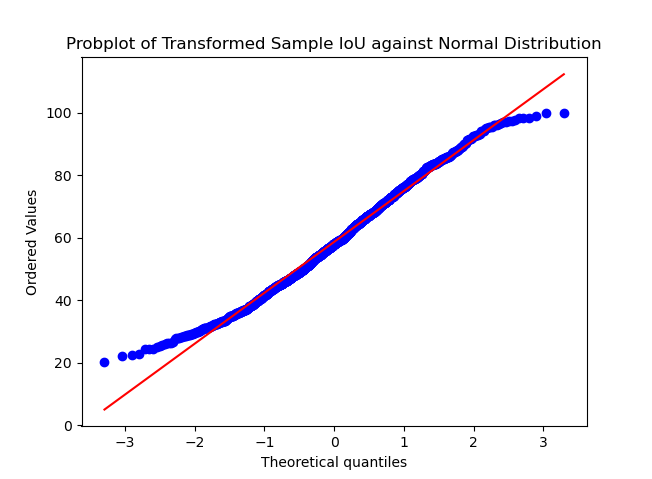
\includegraphics[width=\textwidth]{figures/chap51_time_probplot.png}
		\caption{
			Normal Probability Plot of $X_{trans}$.
		}\label{fig:ch5:sec1:time_probplot}
	\end{subfigure}
	\caption[Sample Transformation $ time $]{
		Transformation of the sample to achieve a normal distribution.
		In a) $X_{raw}$ is shown, which is skewed to the left and not normally distributed.
		The sample is transformed by Equation \ref{equ:trans_time}.
		The result is $X_{trans}$ now shows normal characteristics, as illustrated by the curve of the fitted normal distribution in b).
		The corresponding normal probability plot of $X_{trans}$ is shown in c), which confrims the normal characteristics of $X_{trans}$.
	}\label{fig:ch5:sec1:time_transformation_iou}
\end{figure}




\subsubsection{Hypothesis Testing}

The setting for this hypothesis testing is analog to the previous tests on $IoU$.
In further evaluation the $time_{annot}$ is referred to as $time$, in order to enable a simple distinction between the factors.

First, more general tests are applied on the factors $time_{classical}$ and $time_{dl}$.
The Student's t-test, Kruskal-Wallis test, and Mann-Whitney are performed and their details are presented in Table \ref{tab:ch5:tests_on_time}.
All three tests come to the conclusion to reject $H_{0}$ and accept $H_{A}$.
This proves that the annotation time of \gls{dl} based methods is significantly faster than the annotation time of classical methods, as also illustrated in Figure \ref{fig:ch5:sec1:time_box_plot}.
The information value of this conclusion is especially expressive, due to the application of three different tests with various null hypotheses.

\begin{table}[h!]
	\centering
	\resizebox{\textwidth}{!}{
	\begin{tabular}{l|c c c}
		\toprule 		
		& Student's t-test	& Kruskal-Wallis test 	& Mann-Whitney U-test \\
		\midrule
		data			& $X_{trans}$		& $X_{raw}$ 	 		& $X_{raw}$ 	\\ 
		$H_{0}$			& $\overline{time}_{classical} = \overline{time}_{dl}$ & $med \left( time_{classical} \right)  = med \left( time_{dl} \right)$ & $ten \left( time_{dl} \right) = ten \left( time_{classical} \right)$ 		\\
		$H_{A}$		 	& $\overline{time}_{classical} > \overline{time}_{dl}$ & $med \left( time_{classical} \right) > med \left( time_{dl} \right) $ & $ten \left( time_{dl} \right) \not= ten \left( time_{classical}\right) $ 	\\
		$\alpha$		& $1\%$ 			& $1\%$ 		 		& $1\%$ 		\\ 	
		Statistic		& 28.6792			& 355045	     		& 627.875\\ 
		$\textnormal{\textit{p-value}}$ 
		& $4.8\cdot 10^{-155}$				& $7.2 \cdot 10^{-139}$ & $1.4 \cdot 10^{-138}$ 		\\ 
		$H_{0}$		  	& rejected 			& rejected		 		& rejected 		\\
		\bottomrule
	\end{tabular}}
	\caption[Hypothesis Tests on $ time $]{
		Overview and results of the various statistical test performed on the $ time $.
		The $ time $ is evaluated by various values as the mean, median and tendency of the sample.
		Each factor contains 629 annotations.
		If the $ \textnormal{\textit{p-value}} $ is lower than the significance level $ \alpha $, $ H_{0} $ is rejected and $ H_{A} $ is accepted.
		The same result is achieved by all three different statistical tests, which supports its reliability.
	}\label{tab:ch5:tests_on_time}
\end{table}
% Kruskal-Wallis Test for four factors rejects H0.
Second, the $ time $ is evaluated for the four benchmark methods by the Kruskal-Wallis test.
The null hypothesis 
\begin{equation}
	H_{0}: med \left( time_{Polygon} \right) = med \left( time_{Watershed} \right) = med \left( time_{IOG} \right) = med \left( time_{DEXTR} \right)
\end{equation}
assumes, that the median values do not differ significantly at $ \alpha=1\% $.
$ H_{A} $ states that $ H_{0} $ is not true.
The statistic returns $ \textnormal{\textit{p-value}} = 7.1 \cdot 10^{-141} $, as a result $ H_{0} $ is rejected and $ H_{A} $ accepted.
 
Based on the post analysis by the DSCF test \cite{CF91-dscf}, $ time $ does not differ significantly for the polygon and watershed method based on the median values.
In contrast, the methods \gls{dextr} and \gls{iog} also differ significantly in $ time $ based on the median.

The differences between the factors are illustrated in Figure \ref{fig:ch5:sec1:time_box_plot}.
The \gls{iog} and \gls{dextr} method clearly demonstrate a lower annotation time than the polygon and watershed method.
It is extraordinary to note that for all methods the last quarter of the box plot covers a larger area than the first quarter.
One possible reason is that the different participants spent different amounts of time on particularly complicated objects.
Notable, is that this effect is extreme for the polygon and watershed method, where approximately one quarter spent more than 60 seconds respectively 50 seconds on one annotation. 
This is perhaps caused, due to the possibility for editing is designed more open for these methods and therefore, more time was spent on editing with these these methods, as mentioned at the beginning of this Section.

\begin{figure}
	\centering
	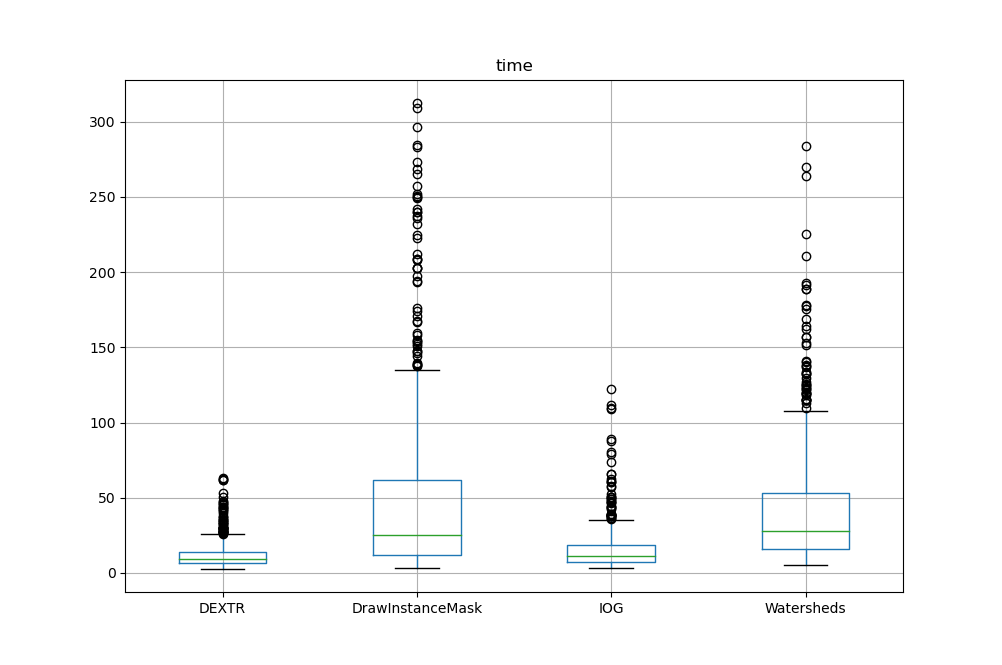
\includegraphics[width=0.9\textwidth]{figures/chap51_time_boxplot.png}
	\caption[Box plots of the methods on $ IoU  $]{
		Box plots of the $ time $ for the four benchmark methods.
		It can be clearly seen, that the required time to perform the \gls{dextr} and \gls{iog} method is lower than for the polygon and watershed method.
		This also applied for the $ med \left( time \right) $ of the single methods, which is statistically confirmed by the Kruskal-Wallis test.
		In general, the polygon and watershed method require a longer annotation time, where the last quarter of the box plot covers a relatively wide range with many outliers. 
		%Despite the difference
	} \label{fig:ch5:sec1:time_box_plot}
\end{figure}


Combining the results of the evaluation from $ IoU $ and the $ time $, it can be said that all methods may achieve an approximately the same level of accuracy.
But the difference between the two types of methods is that, \gls{dl} based method require significantly less time to achieve this state of \gls{iou}.





% !TeX root = ../../main.tex
% Add the above to each chapter to make compiling the PDF easier in some editors.

\section{Watershed}\label{ord:ch5:sec2}

\cite{NS94-Watershed}
\cite{Mey12-WatershedConcept}

\subsection{Method Description}\label{ord:ch5:sec2:subsec1}
Lorem ipsum dolor sit amet, consetetur sadipscing elitr, sed diam nonumy eirmod tempor invidunt ut labore et dolore magna aliquyam erat, sed diam voluptua. At vero eos et accusam et justo duo dolores et ea rebum. Stet clita kasd gubergren, no sea takimata sanctus est Lorem ipsum dolor sit amet. Lorem ipsum dolor sit amet, consetetur sadipscing elitr, sed diam nonumy eirmod tempor invidunt ut labore et dolore magna aliquyam erat, sed diam voluptua. At vero eos et accusam et justo duo dolores et ea rebum. Stet clita kasd gubergren, no sea takimata sanctus est Lorem ipsum dolor sit amet.

\subsection{Architecture}\label{ord:ch5:sec2:subsec2}
Lorem ipsum dolor sit amet, consetetur sadipscing elitr, sed diam nonumy eirmod tempor invidunt ut labore et dolore magna aliquyam erat, sed diam voluptua. At vero eos et accusam et justo duo dolores et ea rebum. Stet clita kasd gubergren, no sea takimata sanctus est Lorem ipsum dolor sit amet. Lorem ipsum dolor sit amet, consetetur sadipscing elitr, sed diam nonumy eirmod tempor invidunt ut labore et dolore magna aliquyam erat, sed diam voluptua. At vero eos et accusam et justo duo dolores et ea rebum. Stet clita kasd gubergren, no sea takimata sanctus est Lorem ipsum dolor sit amet.

\subsection{Refinement}\label{ord:ch5:sec2:subsec3}
Lorem ipsum dolor sit amet, consetetur sadipscing elitr, sed diam nonumy eirmod tempor invidunt ut labore et dolore magna aliquyam erat, sed diam voluptua. At vero eos et accusam et justo duo dolores et ea rebum. Stet clita kasd gubergren, no sea takimata sanctus est Lorem ipsum dolor sit amet. Lorem ipsum dolor sit amet, consetetur sadipscing elitr, sed diam nonumy eirmod tempor invidunt ut labore et dolore magna aliquyam erat, sed diam voluptua. At vero eos et accusam et justo duo dolores et ea rebum. Stet clita kasd gubergren, no sea takimata sanctus est Lorem ipsum dolor sit amet.

\subsection{Results}\label{ord:ch5:sec2:subsec4}
Lorem ipsum dolor sit amet, consetetur sadipscing elitr, sed diam nonumy eirmod tempor invidunt ut labore et dolore magna aliquyam erat, sed diam voluptua. At vero eos et accusam et justo duo dolores et ea rebum. Stet clita kasd gubergren, no sea takimata sanctus est Lorem ipsum dolor sit amet. Lorem ipsum dolor sit amet, consetetur sadipscing elitr, sed diam nonumy eirmod tempor invidunt ut labore et dolore magna aliquyam erat, sed diam voluptua. At vero eos et accusam et justo duo dolores et ea rebum. Stet clita kasd gubergren, no sea takimata sanctus est Lorem ipsum dolor sit amet.
% !TeX root = ../../main.tex
% Add the above to each chapter to make compiling the PDF easier in some editors.

\section{Generalization over users}\label{ord:ch5:sec_3_generalization_user}

% RE-1468
This benchmark study strongly benefits from having real participants applying various methods.
Valuable data is collected, which is, however, challenging to interpret.
This is because participants often have different characteristics as levels of experience, understanding of accuracy, professional background, and motivation.
As a result, the interactive method may be handled differently and the obtained data may vary with respect to various users with different characteristics. 

% Ziel = Methode zu finden mit der alles User gut klarkommen und die über verschiedene user gute Resultate in Zeit und IoU erziehlt.
However, in order to find wide application, an interactive method must work consistently with diverse users.
This section examines the generalization capabilities of the benchmark methods across different users and, therefore, is the counterpart to the previous section.
% Motivation: generalization over user -> an interactive method really performs well and reliable if it delivers good results for all possible users.




\subsection{Benchmark Participants Evaluation}\label{ord:ch5:sec3:subsec1}

In the following the performance of the methods is evaluated over the \getNumberBenchmarkParticipants participants.
In contrast to the previous evaluation, here the benchmark runs performed by the colleagues, who are working on this topic, are excluded.
This is done intentionally, in order to not distort the evaluation, since the users are explicitly evaluated here and the data obtained from most experienced users would be biased.

In order to evaluate the generalization capabilities across multiple users, first statistical key figures as the mean and standard deviation $ \sigma $ are evaluated.
The combined mean and $ \sigma $ for the participants are presented in Table \ref{tab:ch5:all_benchmark_users_varaince}.
% For IoU low std-dev, but for time vergleichsweise hoch 
It can be observed, that $ \sigma_{IoU} $ is very similar for the benchmark methods and only ranges from $ \sigma_{IoU} = 0.1187 $ for \gls{dextr} to $ \sigma_{IoU} = 0.1669 $ for watershed.
In contrast $ time $ shows a strong deviation, with $ \sigma_{time} = 15.0977 $ for \gls{dextr} the deviation is less than half as large as for polygon with $ \sigma_{time} = 39.0214 $.
The mean value is presented to put $ \sigma $ into context.
A graphical illustration of the deviation of $ IoU $ and $ time $ is already presented in the box plots from Figure \ref{fig:ch5:sec1:iou_box_plot} and \ref{fig:ch5:sec1:time_box_plot}.
Further, these results support the conclusion of Subsection \ref{ord:ch5:sec1:subsec2} and \ref{ord:ch5:sec1:subsec3}, which state that in terms of $ IoU $ the methods perform approximately equal, while $ \overline{time} $ and $ med(time) $ do differ significantly between the \gls{dl} based and classical benchmark methods.
% Calculate the variance for time and iou.
\begin{table}[h!]
	\centering
	\begin{tabular}{l|c c c c}
		\toprule 		
			 				& $ Polygon $  	& $ Watershed $ 	& $ DEXTR $ 	& $ IOG $	\\
		\midrule
		\rule{0pt}{3ex}%  EXTRA vertical height  
		$ \overline{IoU} $	& 0.8066 		& 0.8166		 	& 0.8543		& 0.8020	\\
		\rule{0pt}{3ex}%  EXTRA vertical height  
		$ \sigma_{IoU} $	& 0.1287 		& 0.1669		 	& 0.1187 		& 0.1559	\\
		\rule{0pt}{3ex}%  EXTRA vertical height  
		$ \overline{time} $	& 34.399 		& 45.076			& 14.542 		& 18.059	\\
		\rule{0pt}{3ex}%  EXTRA vertical height  
		$ \sigma_{time} $	& 39.021 		& 37.796			& 15.098 		& 17.383	\\
		\bottomrule
	\end{tabular}
	\caption[Mean and standard deviation of the benchmark methods]{
		Presentation of the mean and standard deviation $ \sigma $ for $ IoU $ and $ time $.
		It can be seen that $ \sigma_{IoU} $ stays almost constant over the benchmark methods.
		In contrast, $ \sigma_{time} $ differs between the methods.
		The mean value was given for IoU and time to better interpret $ \sigma $.
	}\label{tab:ch5:all_benchmark_users_varaince}	
\end{table}
% TODO Mir fehlt hier irgendwie eine genauere Angabe was das für Werte sind. In diesem Kapitel geht es doch um die User?     Irgendwo (vllt auch als Formel) sollte gezeigt werden, dass hier ein Mittel über die User-weisen Mittel (mean_mean_IoU_per_user_per_method) gebildet wird.     Genauso ist das wohl die mittlere Varianz (gemittelt über die User), oder?


To get even deeper insights about the generalization across different users, in Figure \ref{fig:ch5:sec3:all_benchmark} box plots for $ IoU $ and $ time $ are shown for all participants individually.
Here, no statistical tests for equality within the methods were performed, because the visualization already indicates that there are strong deviations between the user for each method.
The variations between the individual users are present in all methods and most likely due to the varying characteristics of the users as introduced in the beginning of this section.
% \eg different experience levels, how , and how well a user got along with the method.

However, it can be stated that for $ IoU $ \gls{dextr} has the smallest deviation and is the most constant method over all participants, while the other methods still perform similar.

% Box plot of all BenchmarkParticipants (not experienced user aka me)
\begin{figure} 
	\centering
	\begin{subfigure}[t]{1.0\textwidth}
		\centering
		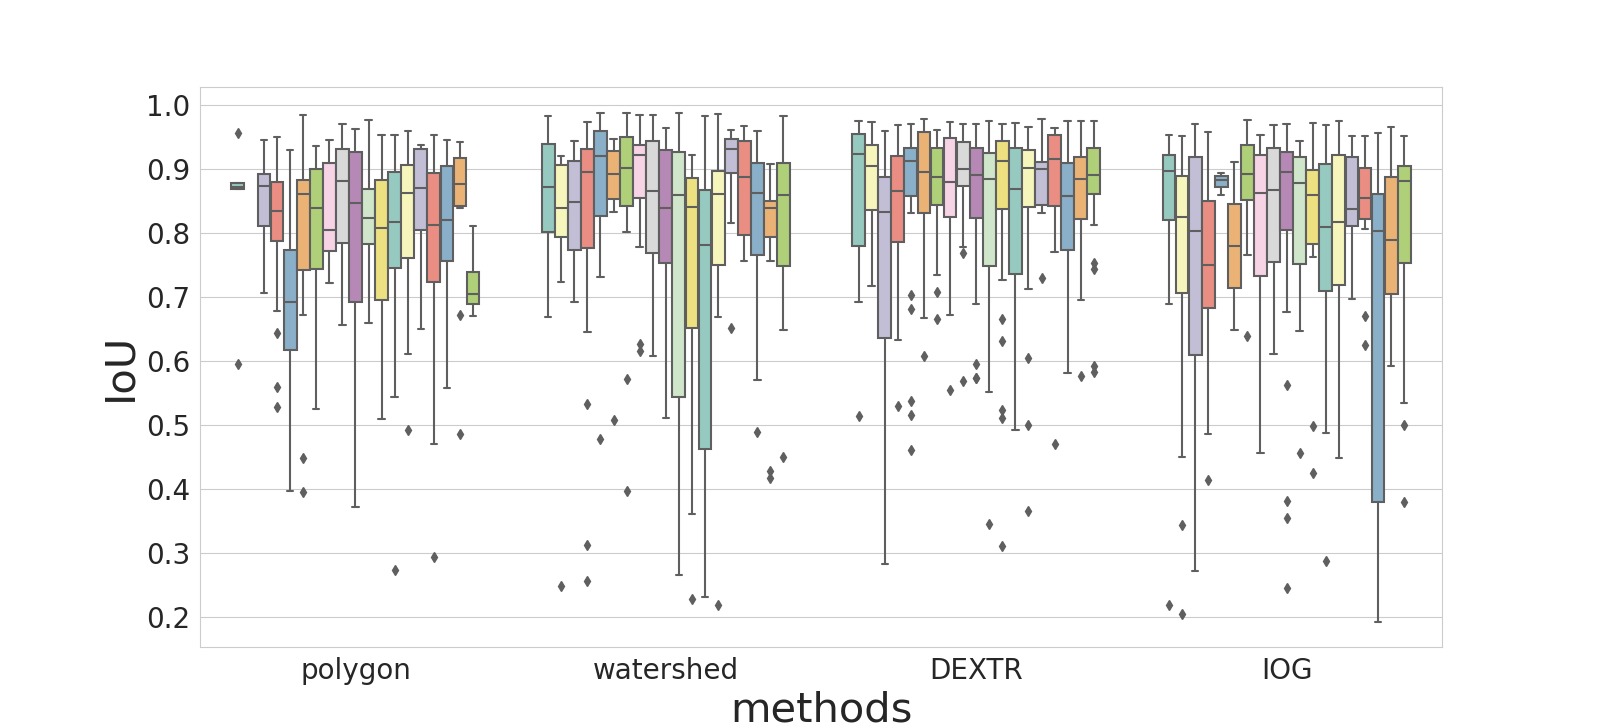
\includegraphics[width=\textwidth]{figures/chap53_all_users_iou.png}
		\caption{
			The \gls{dextr} delivers mostly constant $ IoU $ values with some outliers, while the other methods are mostly characterized by irregularities.
		}\label{fig:ch5:sec3:all_benchmark_iou}
	\end{subfigure}
	\\
	\begin{subfigure}[t]{1.0\textwidth}
		\centering
		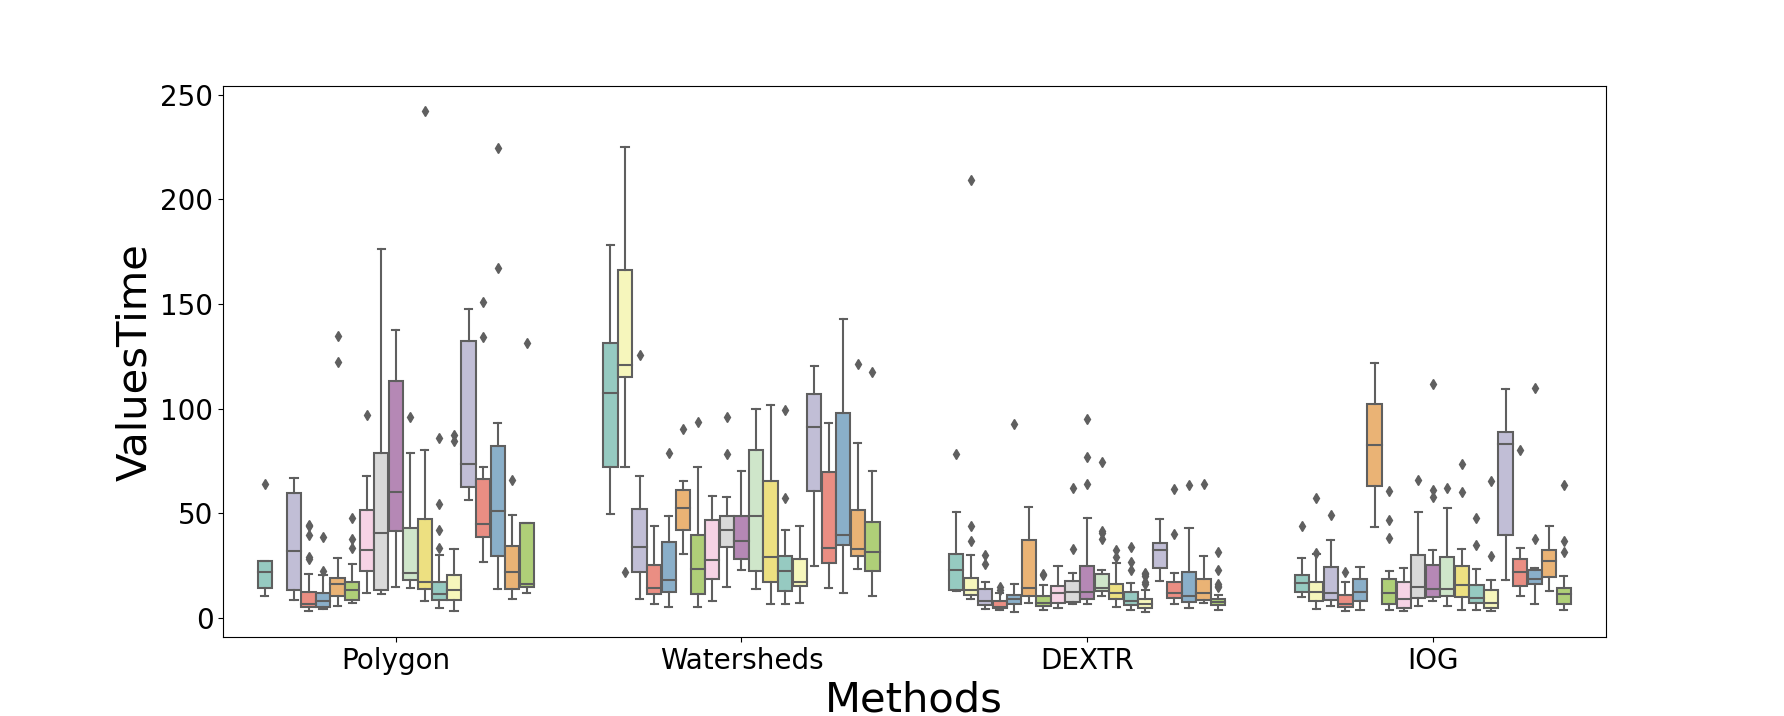
\includegraphics[width=\textwidth]{figures/chap53_all_users_time.png}
		\caption{
			For $ time $ the \gls{dextr} method convinces with a mostly constant performance, while the \gls{iog} method has two users who are the exception to the consistency.
			In contrast for the polygon and watershed method consistency over various user is not given.			
		} \label{fig:ch5:sec3:all_benchmark_time}
	\end{subfigure}
	\caption[Box plots of benchmark participants on $ IoU $ and $ time$.]{		
		The box plots of $ IoU $ and $ time $ over the \getNumberBenchmarkParticipants benchmark participants.
		The single box plots indicate how the methods performed over the single users, the order of the users is the same for both figures. 
		Large differences between the box plots within a method indicate poor generalization capabilities and vice versa.
	}\label{fig:ch5:sec3:all_benchmark}
\end{figure}

In terms of $ time $ the \gls{dl} based methods show less variance over the users than the classical methods.
The \gls{dextr} method performs best, while the \gls{iog} method has two bigger outliers.
The difference between \gls{dl} based and classical methods is partly caused by the design of the methods, which guides the user more or less.
On the one side, the polygon and watershed method do little to guide the user,
but give the user a lot of freedom when performing the label task.
This room for interpretation is used differently by the users, which leads to different label times and, therefore, higher variance.
On the other side, the \gls{dextr} and \gls{iog} method provide strong guidance by defining the amount of clicks required for an initial prediction.
Although the application of refinement is still possible, this prevents users from spending too much time on an initial prediction.
This strong guidance of the user while applying the method leads to a more constant annotation time and thereby a lower variance in $ time $.
% polygon and watershed are more freely

In conclusion, for $IoU$ the \gls{dextr} method generalizes best over multiple users, while the other models do no achieve a constant performance over various users.
For $ time $ it is observed, that methods with strong guidance as \gls{dextr} and \gls{iog} are more constant in $ time $, than the polygon and watershed method, that are designed more open and, therefore, allow higher variance.


\subsection{Two Experienced Users} \label{ord:ch5:sec3:subsec2_cmo_afe}

Normally, the participants have labeled only a part of the benchmark images. 
In the following, eight benchmark runs are evaluated where all benchmark images were labeled by two users who have more experience working on this topic.
Although only two different users are compared with each other, the significance is given, since all images of the benchmark were labeled.
However, it must be mentioned that the experience level of both users is not the same, because $ \textnormal{\textit{User 2}} $ is more trained than $ \textnormal{\textit{User 1}} $.

% No significant difference in the IoU between the two user could be detected -> generalize well over various users (few user, large data)
For the $ IoU $, the box plots in Figure \ref{fig:ch5:sec3:cmo_afe_iou} indicate, that the $ IoU $ is more or less equal fors $ \textnormal{\textit{User 1}} $ and $ \textnormal{\textit{User 2}} $ for the four benchmark methods.
The equality of the obtained values from both users are statistically confirmed by the Kruskal-Wallis test, the details of the tests are presented in Table \ref{tab:appendix:afe_cmo_kruskal_wallis_iou}.

An equivalent analysis was performed for $ time $, as presented in Figure \ref{fig:ch5:sec3:cmo_afe_time}.
Interestingly, here the annotation time between $ \textnormal{\textit{User 1}} $ and $ \textnormal{\textit{User 2}} $ differs strongly for polygon and watershed, while the annotation time is very similar for \gls{dextr} and \gls{iog}.
The statistical relevance of this observation is again confirmed by the Kruskal-Wallis test, presented in detail in Table \ref{tab:appendix:afe_cmo_kruskal_wallis_time}.

\begin{figure} [h!]
 	\centering
 	\begin{subfigure}[t]{0.45\textwidth}
 		\centering
 		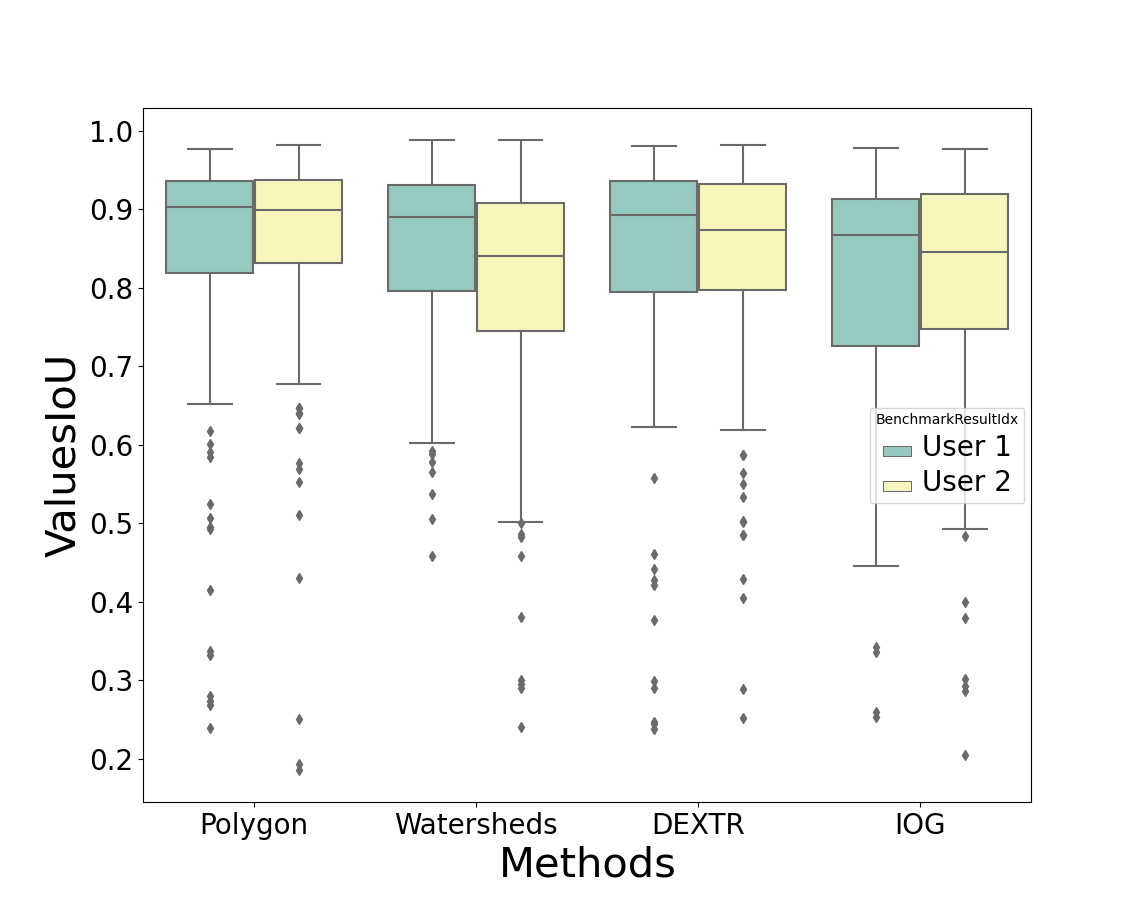
\includegraphics[width=\textwidth]{figures/chap53_afe_cmo_iou.png}
 		\caption{
 			Box plots of the $ IoU $ for the four benchmark methods of $ \textnormal{\textit{User 1}} $ and $ \textnormal{\textit{User 2}} $.
 			The visualization does not indicate any significant difference in $ IoU $.
 		} \label{fig:ch5:sec3:cmo_afe_iou}
 	\end{subfigure}
 	\hfill
 	\begin{subfigure}[t]{0.45\textwidth}
 		\centering
 		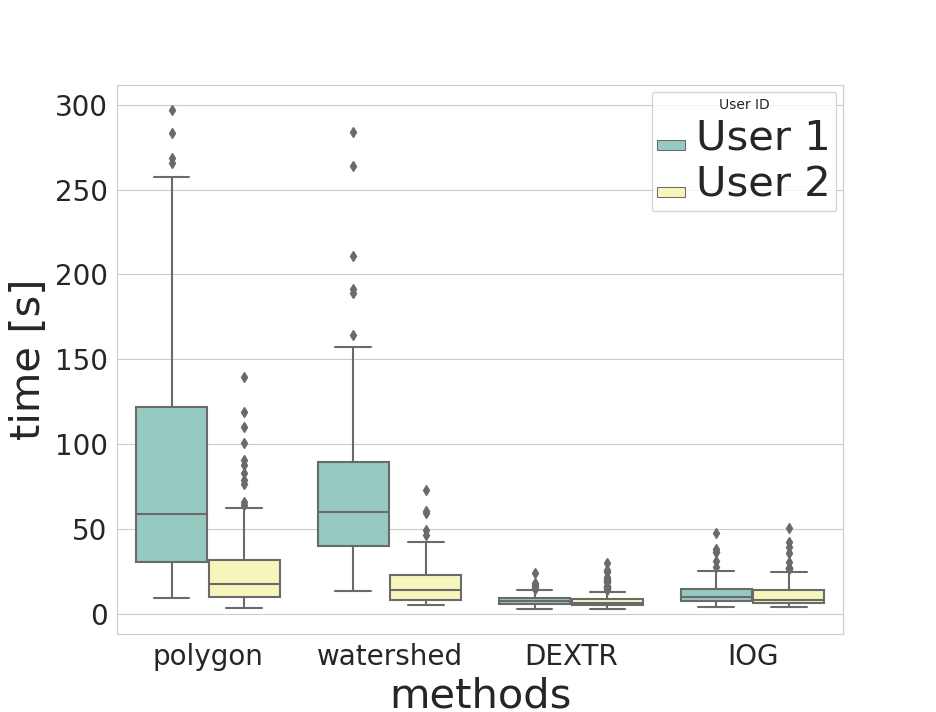
\includegraphics[width=\textwidth]{figures/chap53_afe_cmo_time.png}
 		\caption{
 			Box plots of the $ time $ for the four benchmark methods of $ \textnormal{\textit{User 1}} $ and $ \textnormal{\textit{User 2}} $.
 			A significant difference in $ time $ for the polygon and watershed is shown, while the \gls{dextr} and \gls{iog} methods perform similar.
 		}\label{fig:ch5:sec3:cmo_afe_time}
 	\end{subfigure}
 	\caption[Box plots of two experienced user on $ IoU $ and $ time$.]{		
 		These two figures show the comparison of the two users over the benchmark methods based on $ IoU $ and $ time $.
 		The hypothesis based on the graphical visualizations are statistically supported by the Kruskal-Wallis test as presented in detail in Table \ref{tab:appendix:afe_cmo_kruskal_wallis_iou} and \ref{tab:appendix:afe_cmo_kruskal_wallis_time}.
 	}\label{fig:ch5:sec3:cmo_afe}
\end{figure}

% User 2 more experienced that User 1
This large difference for Polygon and Watershed was not expected, but it emphasizes again how large the variance can be between different users who achieve the same performance.
This difference may be partly caused by the different level of experience of the two users.
Anyway, it is not surprising that this occurs for the classical methods, that are more freely interpretable and, therefore, leave the user a more open application.
Rather this supports the conclusion of the previous subsection, that methods with stronger guidance perform more consistent in the annotation time.


\subsection{Simulations With Different Click Patterns}\label{ord:ch5:sec3:subsec3}
% RE-1468

% Simulations are easily scalable, faster and cheaper than the acquisition of manual clicks from real users.
% Second, in a simulation no variance occurs between the set clicks of various users, if the.
% Third, simulations have the possibility to effortless create various click patterns, that \eg vary the set click by a random offset, in order to simulate a various types of user behavior.
%On the other hand, simulations are only capable to replicate the user's behavior to a certain extent.
% Further, the involvement of human users is especially important for methods, which performance depends on user interactions.


In order to gain deeper insights on the functionality of the \gls{dextr} and \gls{iog} method the simulation setup is modified.
% Motivation - Nachahmung von unterschiedlichen Usertypen durch unterschiedliche Genauigkeit bei der Klick-Simulation.
The altered simulation setup uses different levels of accuracy, to simulate more realistic user clicks.
% Simulation of with different permutation / deviation / - simulation of different user

The level of accuracy is defined by a deviation of maximal $ n_{deviation} $ \Unit{px}.
In the range $ \left[-n_{deviation}, \dots, 0, \dots, n_{deviation} \right] $ two values are randomly selected and added to the ideal row and column.
This random factor was added, to simulate the varying accuracy of single user clicks.
The smaller $ n_{deviation} $, the more accurate are the simulated clicks.
In the simulation first the ideal click position is calculated and further the random deviation is added.
This procedure is applied to the extreme points of the \gls{dextr} method and to the foreground and background clicks of the \gls{iog} method.
\begin{table}[h!]
	\centering	
	\resizebox{\textwidth}{!}{
	\begin{tabular}{l l|c c c c c c c}
		\toprule
				&						& \multicolumn{7}{c}{mIoU} \\
				& {$ n_{deviation} $} 	& 0	\Unit{px}	& 5	\Unit{px}	& 10 \Unit{px}	& 15 \Unit{px}	& 20 \Unit{px}	& 25 \Unit{px}	& 30 \Unit{px}	\\
		\midrule
		DEXTR 	& PASCAL (VP \cmark)	& 0.9103	& 0.8323	& 0.7626	& 0.7032 	& 0.6479	& 0.6047	& 0.5626		\\
				& PASCAL (VP \xmark)	& 0.7807	& 0.7523	& 0.7019	& 0.6543 	& 0.6085	& 0.5695	& 0.5317		\\
				& Benchmark				& 0.8414	& 0.7743	& 0.6887	& 0.6240 	& 0.5579	& 0.5027	& 0.4892		\\
		\midrule
		IOG 	& PASCAL (VP \cmark)	& 0.9267	& 0.8846	& 0.8092	& 0.7352 	& 0.6578	& 0.5953 	& 0.5457		\\
				& PASCAL (VP \xmark)	& 0.8081	& 0.7720	& 0.7099	& 0.6476 	& 0.5979	& 0.5337	& 0.4873		\\
				& Benchmark				& 0.8219	& 0.7865	& 0.7173	& 0.6027 	& 0.5268	& 0.4493 	& 0.4058		\\
		\bottomrule
	\end{tabular}}
	\caption[Simulations with different click patterns]{
		Simulations of the \gls{dextr} and \gls{iog} method with user clicks, that are simulated with varying degrees of accuracy.
		The parameter $ n_{deviation} $ states the maximal possible deviation from the optimal point, in order to mimic different types of users.
		As expected, the performance decreases with increasing deviation in the simulated user clicks.
	}\label{tab:ch5:simulation_various_click_patterns}
\end{table}

The performance constantly decreases with higher $ n_{deviation} $, as demonstrated in Table \ref{tab:ch5:simulation_various_click_patterns}. 
Even a comparable small deviation of maximal 5 \Unit{px} leads a notable drop in performance \eg from $ mIoU = 0.9103 $ to 0.8323 for \gls{iog} on the PASCAL \gls{voc} dataset with the application of \gls{vp}.
This factor needs to be taken into account, if these methods are applied by real users.





% !TeX root = ../../main.tex
% Add the above to each chapter to make compiling the PDF easier in some editors.

\section{Survey Evaluation}\label{ord:ch5:sec4_survey}
% RE-1469
After participating in the benchmark study 17 users also filled out the post survey.
This survey consists out of five questions, to gain deeper insights on the user's experience.
The questions and their results are presented in \ref{fig:ch5:sec4:suvery}.
% Soft Factors
% Useability

\begin{figure}
	\centering
	\begin{subfigure}[t]{0.48\textwidth}
		\centering
		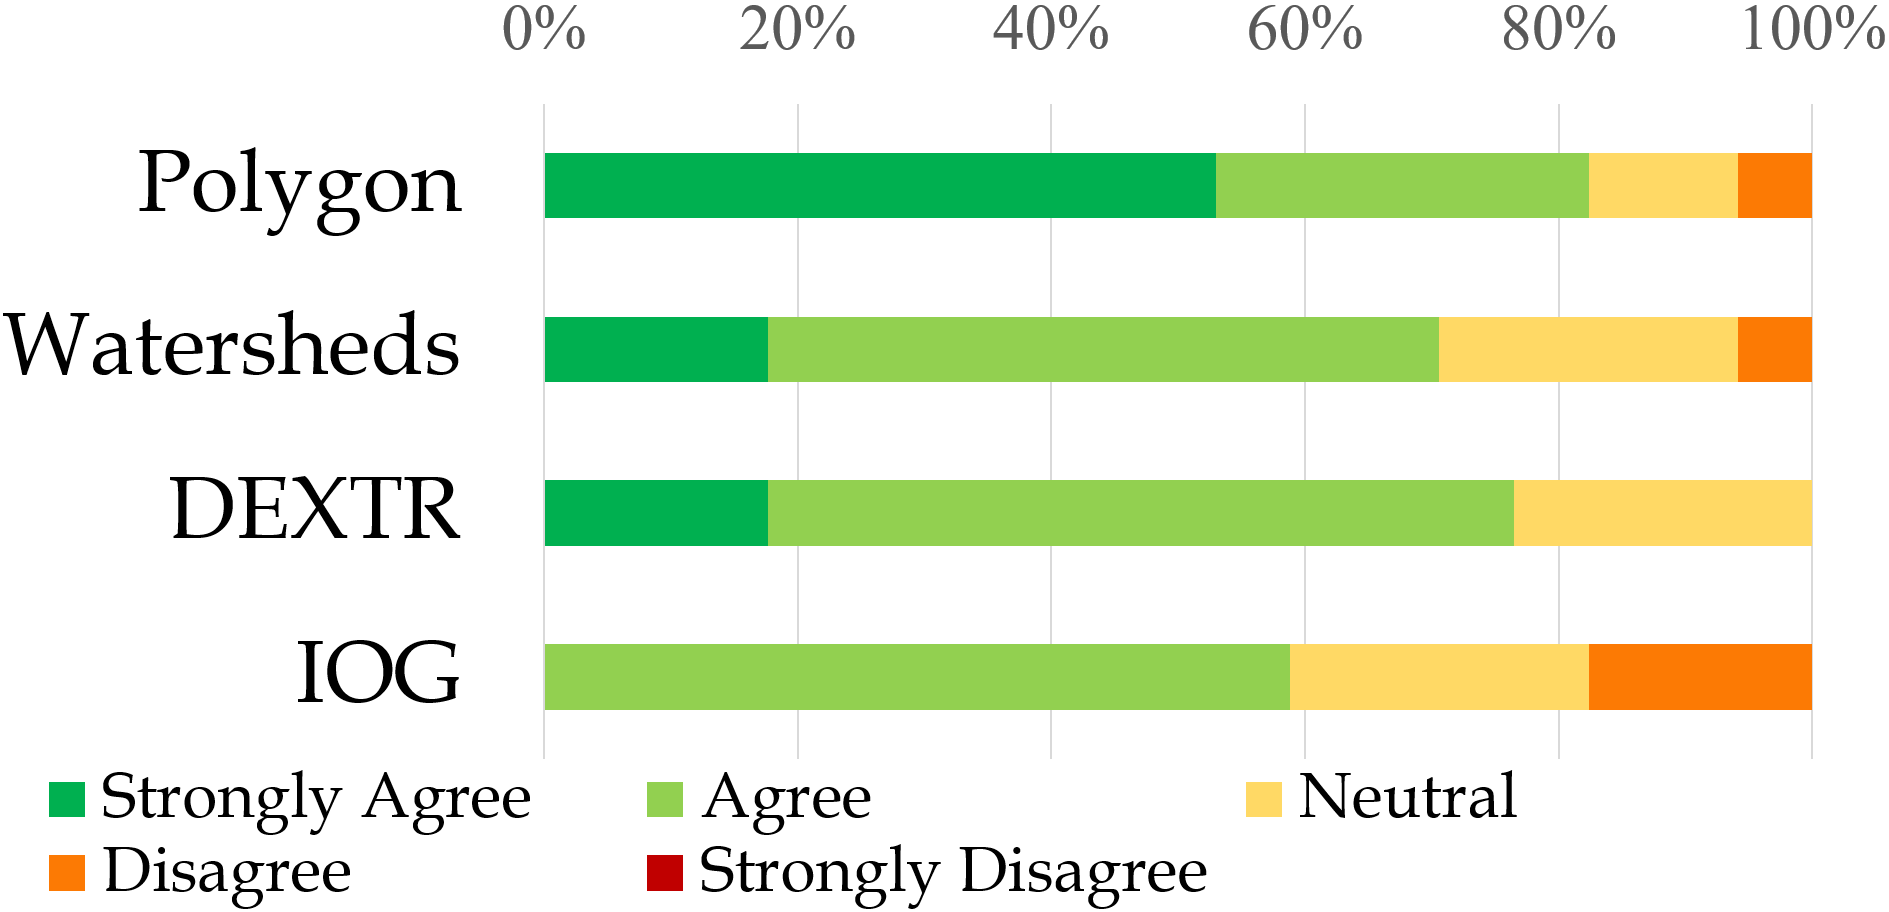
\includegraphics[width=\textwidth]{figures/chap54_q1.png}
		\caption{
			Question 1: \textit{The result / prediction masks of the method were as I expected them to be.}
		} \label{fig:ch5:sec4:q1}
	\end{subfigure}
	\hfill
	\begin{subfigure}[t]{0.48\textwidth}
		\centering
		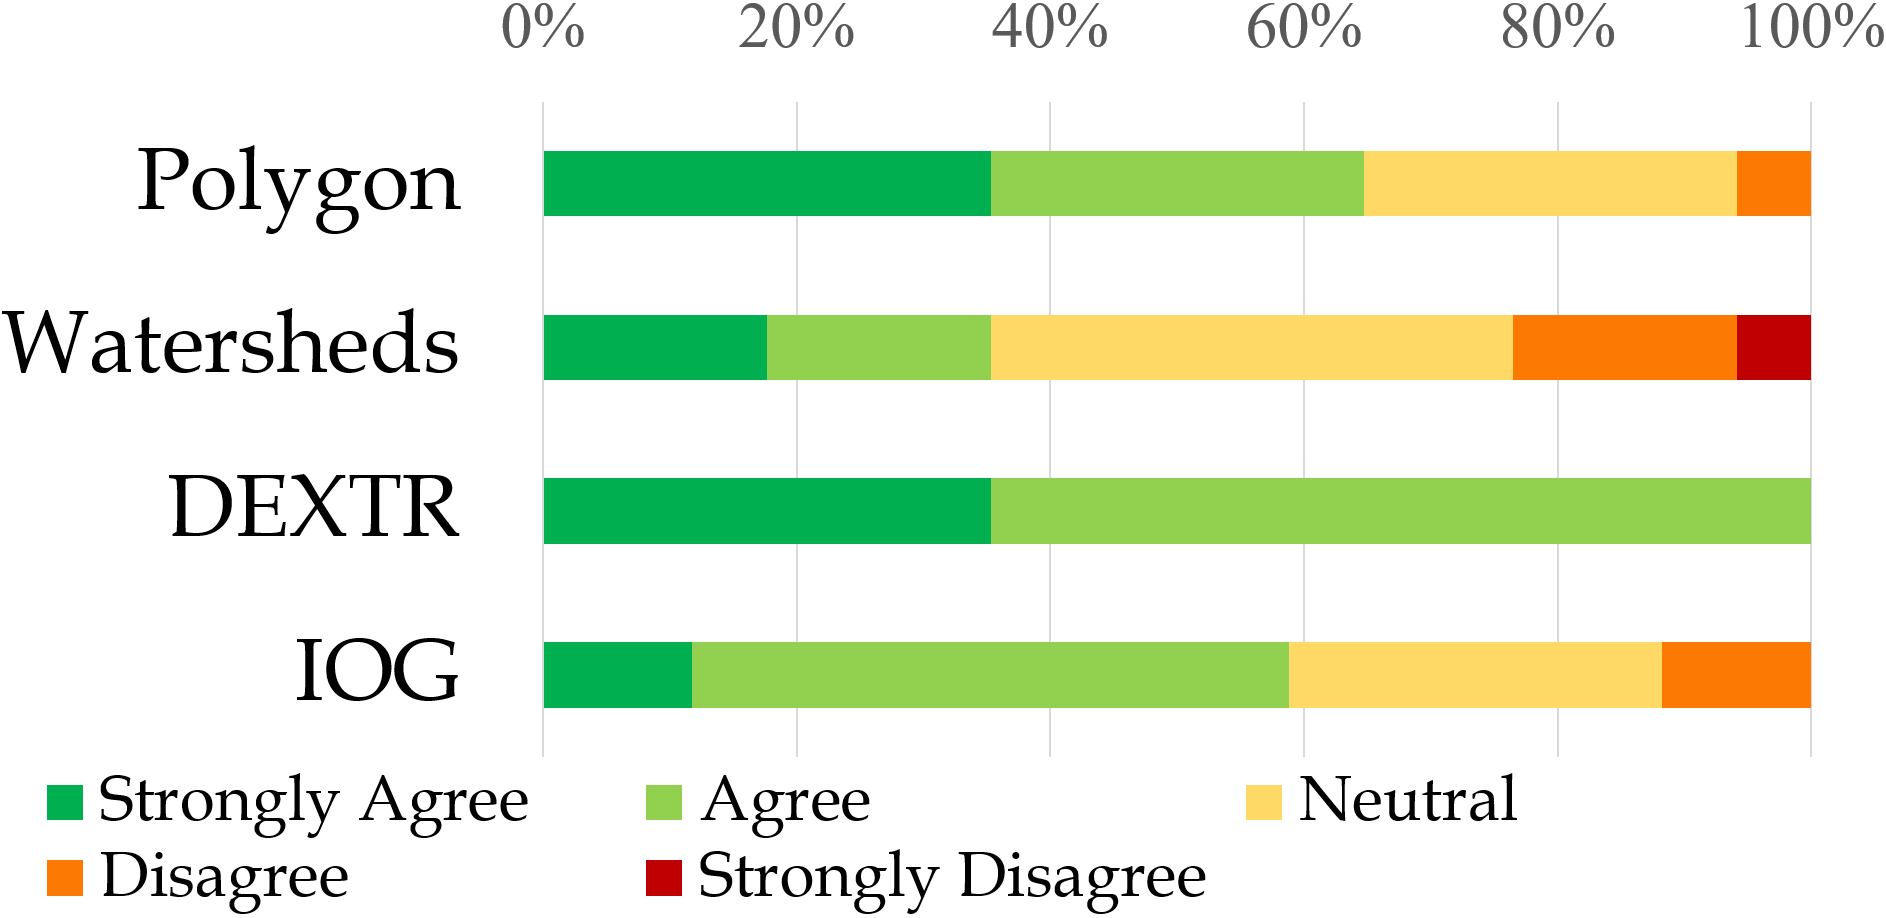
\includegraphics[width=\textwidth]{figures/chap54_q2.png}
		\caption{
			Question 2: \textit{I was satisfied with the result / prediction masks.}
		} \label{fig:ch5:sec4:q2}
	\end{subfigure}
	\\
	\begin{subfigure}[t]{0.48\textwidth}
		\centering
		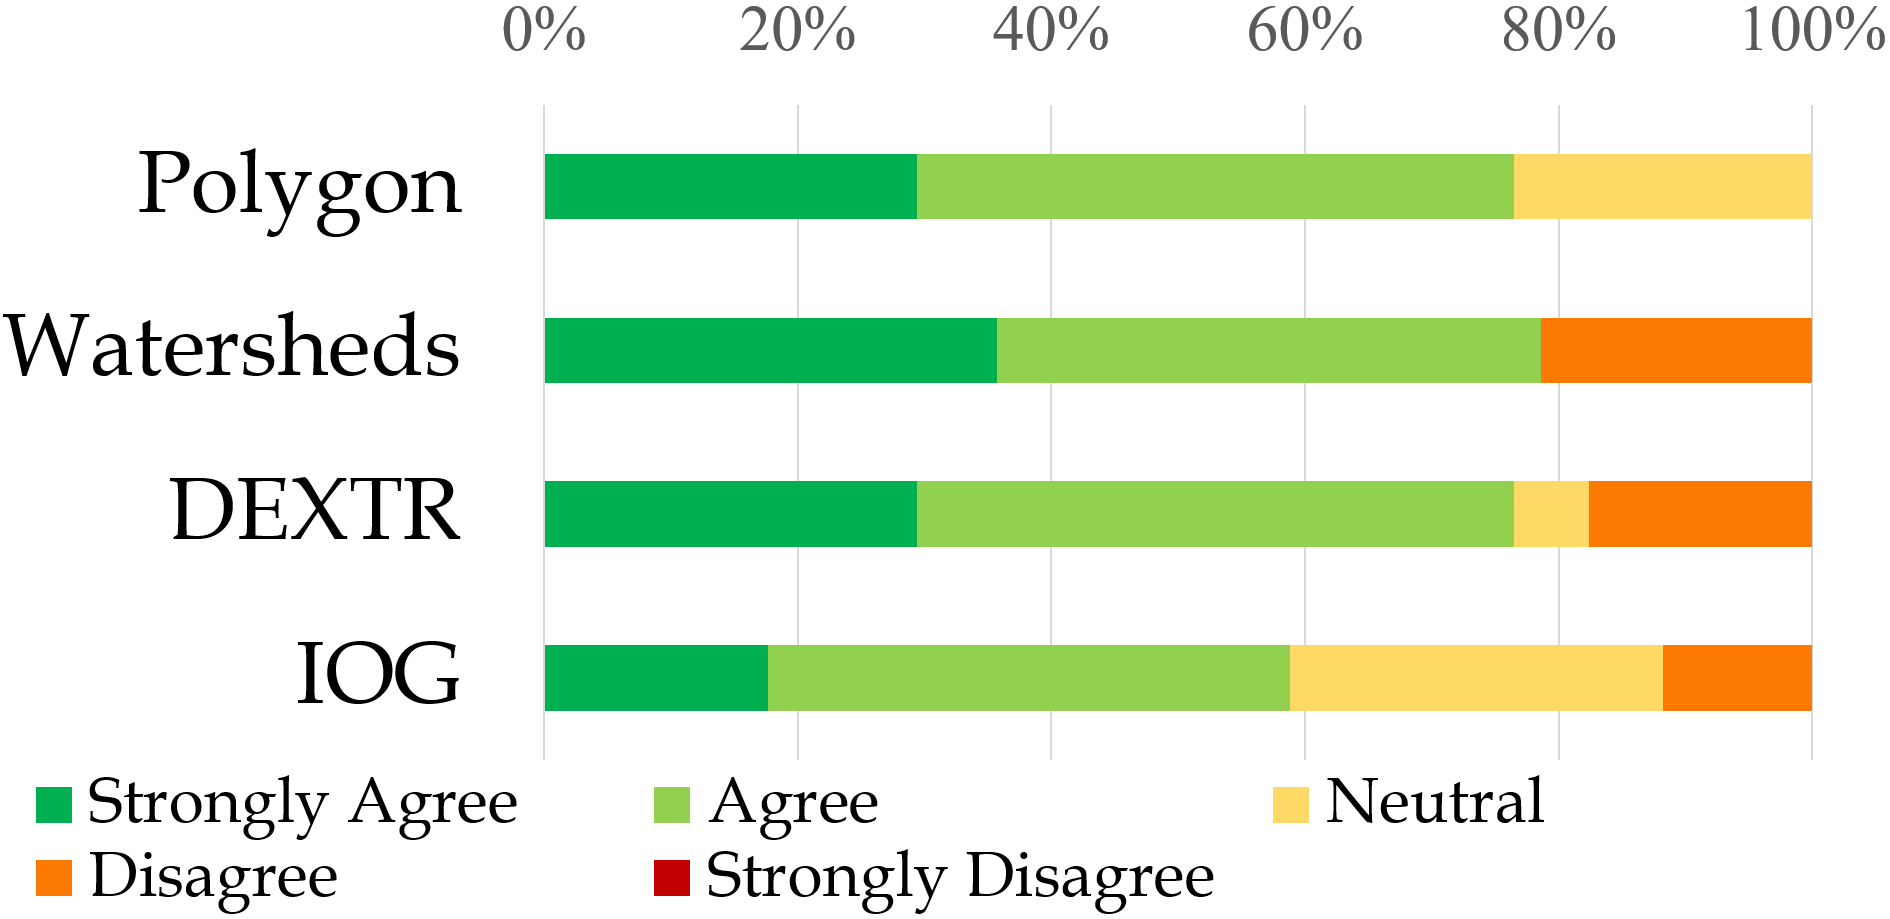
\includegraphics[width=\textwidth]{figures/chap54_q3.png}
		\caption{
			Question 3: \textit{With more experience / time in the labeltool I became better at handling the method and applying it.}
		} \label{fig:ch5:sec4:q3}
	\end{subfigure}
	\hfill
	\begin{subfigure}[t]{0.48\textwidth}
		\centering
		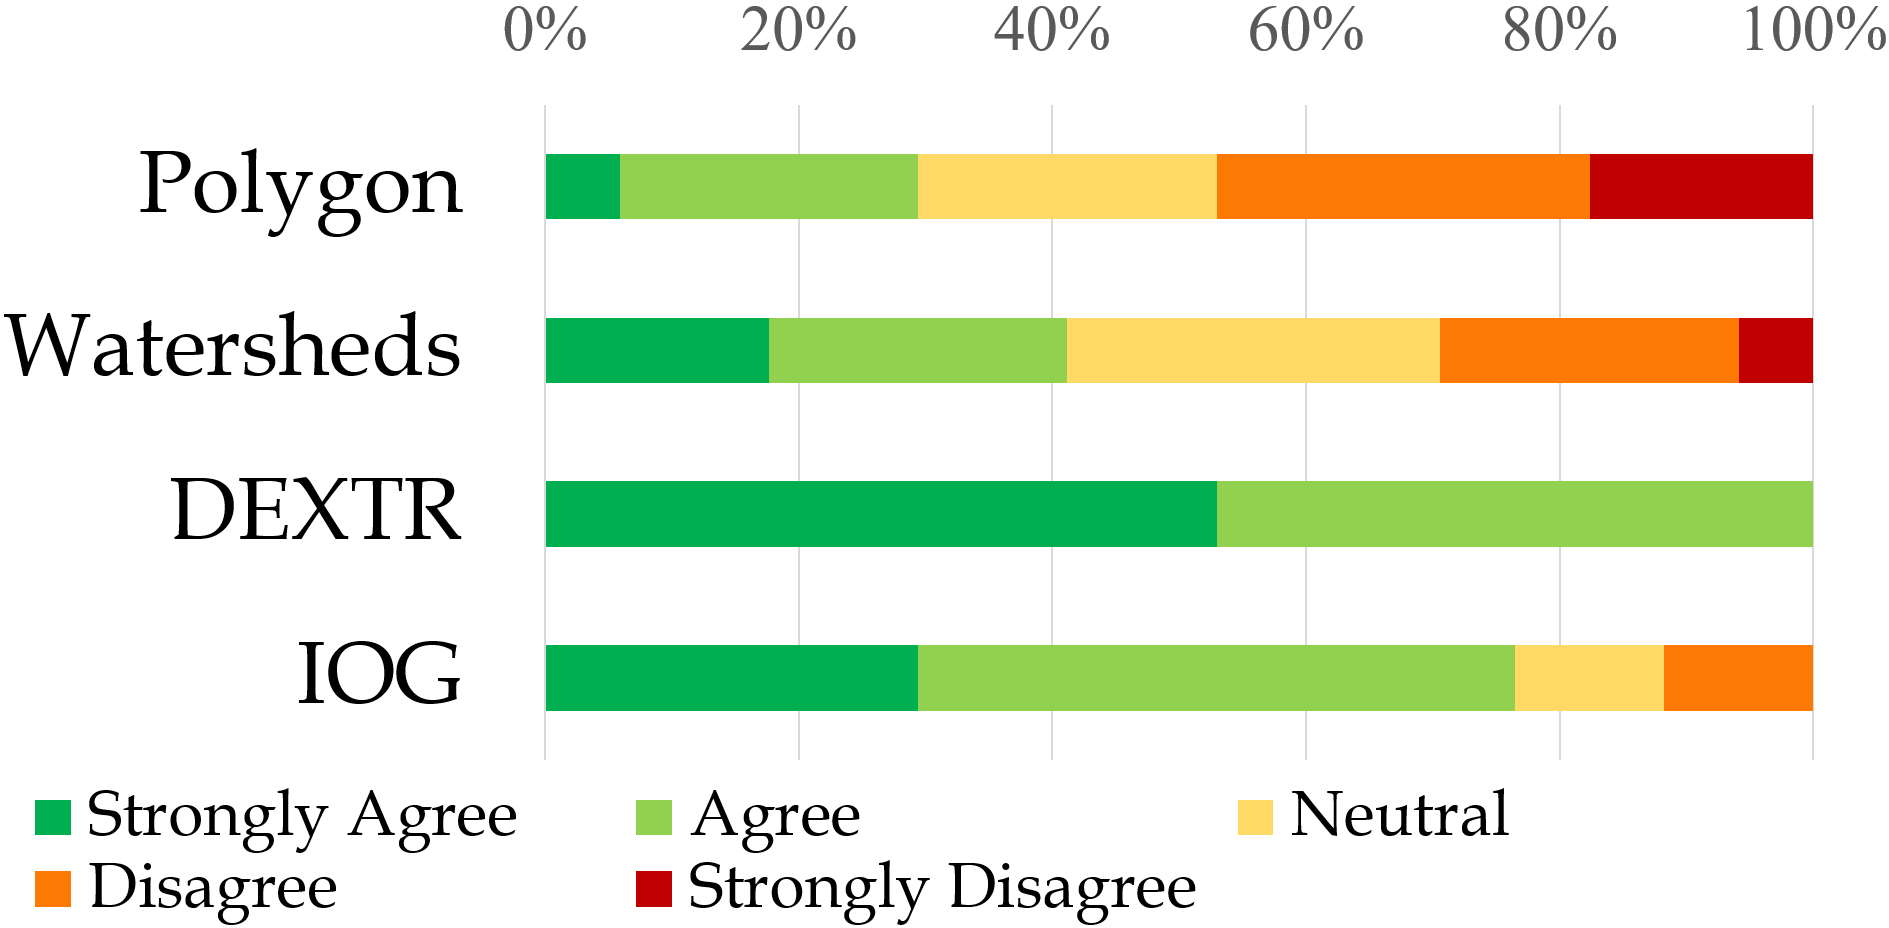
\includegraphics[width=\textwidth]{figures/chap54_q5.png}
		\caption{
			Question 4: \textit{It was ‘fun’ / ‘exciting’ to use the method.}
		} \label{fig:ch5:sec4:q4}
	\end{subfigure}
	\\
	\begin{subfigure}[t]{0.48\textwidth}
		\centering
		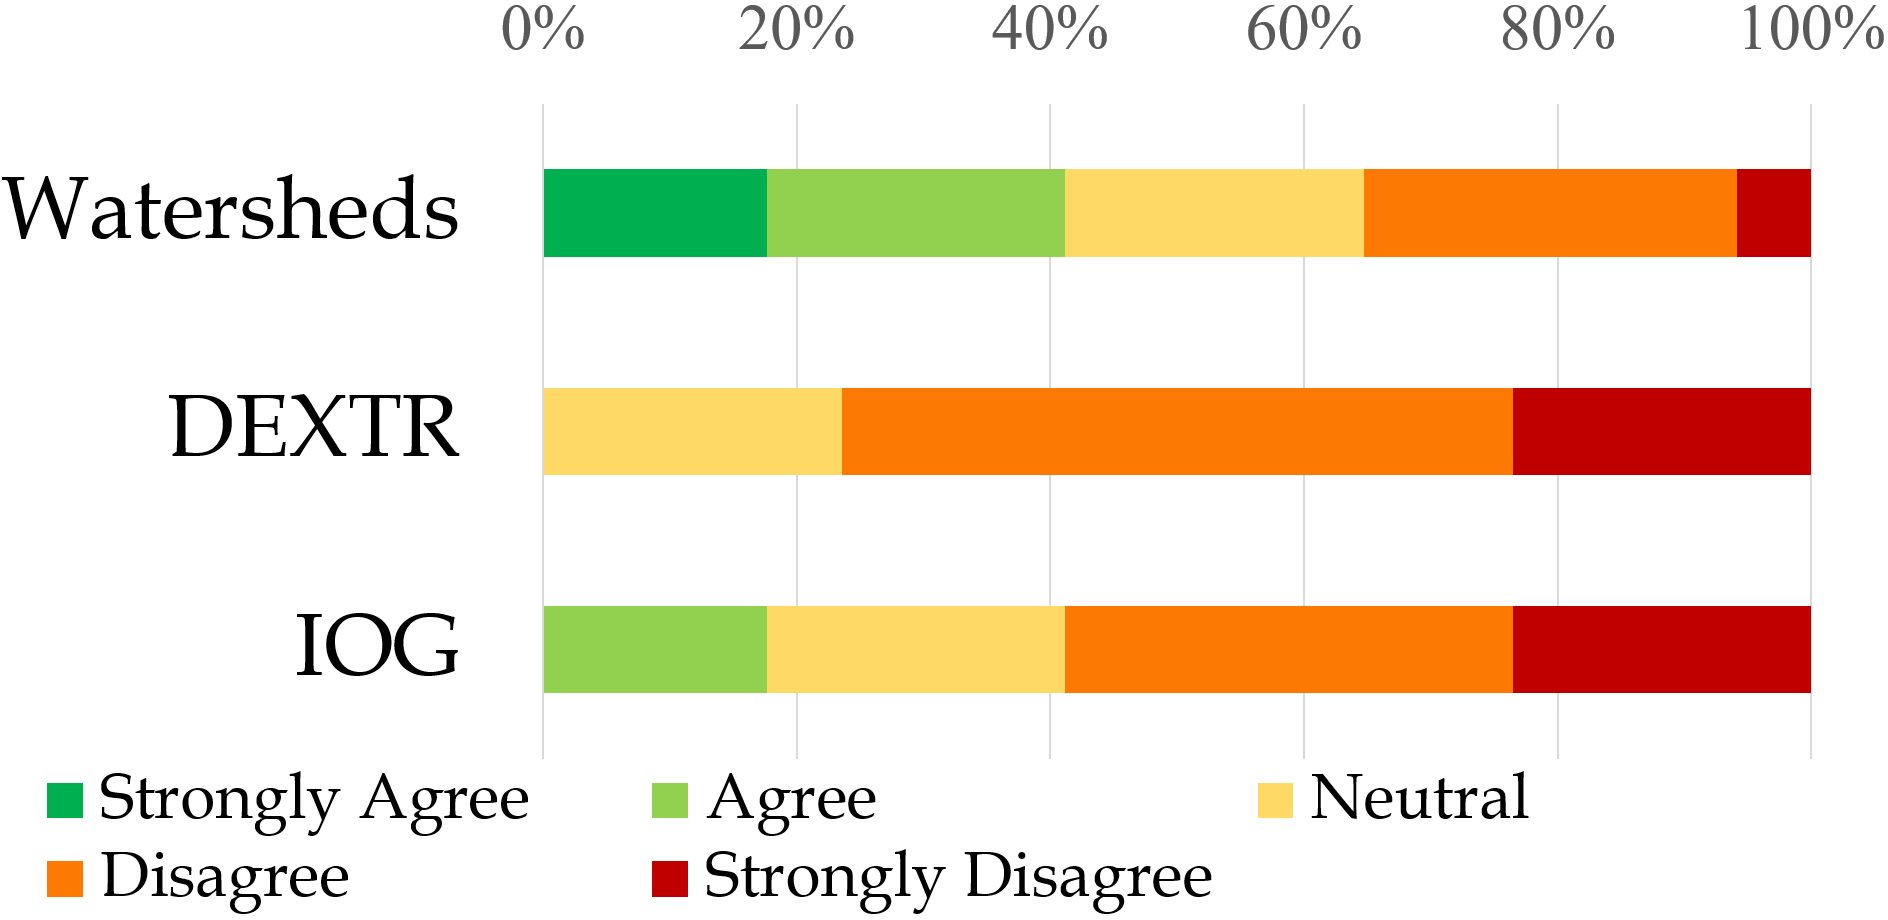
\includegraphics[width=\textwidth]{figures/chap54_q4.png}
		\caption{
			Question 5: \textit{By manually drawing a polygon I could achieve a better result in the same time.}
		} \label{fig:ch5:sec4:q5}
	\end{subfigure}
	\caption [Watershed User Interaction]{
		Responses on the questions from the survey.
		The answer options for all question are \textit{Strongly Agree}, \textit{Agree}, \textit{Neutral}, \textit{Disagree}, and \textit{Strongly Disagree}.
	} \label{fig:ch5:sec4:suvery}
\end{figure}
% TODO update proper figure if approved

In order to be accepted by an user a method needs to be understandable and create deterministic results.
When the method performs as intended, a pleasant user experience is created, while frustration is caused otherwise.
These factors are investigated in the questions one and two, which represent that all methods perform as the user expects and the users are mostly satisfied with the result.

Further, in question 3 and 5 it was researched whether the user was time efficient and improved over time.
A review of the total experience and the pleasantly of the application is asked in Question 4.
Here the \gls{dl} based methods received good feedback.
This reasons in their little user interaction and excitement of applying novel methods.

In conclusion, based on this survey the \gls{dextr} method seems to provide the best user experience.
Manual methods like polygon drawing or Watersheds also serve good results, but are not time efficient and pleasant to apply, compared to the \gls{dextr} and \gls{iog} method.  

% !TeX root = ../../main.tex
% Add the above to each chapter to make compiling the PDF easier in some editors.

\section{Suitability Of DEXTR and IOG Annotations For Training} \label{ord:ch5:sec5_retrain}
% RE-1470
In this section it is examined if annotations created by the \gls{dextr} and \gls{iog} method are suitable to train a new \gls{dl} model for semantic segmentation. %TODO or instance segmentation?
In the following the experimental setup is described in three stages: creation of annotations, model training, and model evaluation.
 
% Create annotations.
As first step, simulations are applied to create the required user input for the \gls{dextr} and \gls{iog} method.
The resulting predictions from the models are treated as new labels $ \textbf{Y}_{new} $. 
The simulation is performed with one refinement click for \gls{dextr} and four refinement clicks for \gls{iog}.
Further, the simulation setup is without mayor randomization, as described in Subsection \ref{ord:ch5:sec2:subsec2}.
The simulation is performed on the training split of the MVTec \gls{d2s} dataset \cite{Paddo18-D2S}, the test split is not altered.
Thereby, two variants of the \gls{d2s} dataset are used, in the training split the normal version of has 4380 images and 6900 annotations, while the augmented version contains 14380 images and 83337 annotations.
The goodness of the newly created annotations $ \textbf{Y}_{new} $ is at least at 0.91 \gls{miou}, as presented in Table \ref{tab:ch5:results_annot_usability}.

% Train model.
In the second step, the new annotations $ \textbf{Y}_{new} $ of the train split, are used to train semantic segmentation models $ m $.
As backbone of a model the Mask-RCNN \cite{He17-MaskR-CNN} is used, which is pretrained on the COCO dataset \cite{Lin14-Coco}.
All trainings are performed with the same settings, to enable a fair comparison.
A training lasts $ n_{epochs} = 30 $ epochs, with the learning rate $ \lambda = 0.001 $ and \gls{sgd} optimizer \cite{Ruder16-SGD}.
To establish a benchmark for comparison, also two models are trained on the original \gls{gt} of the normal and augmented \gls{d2s} dataset.
The models itself do not contain any novelty, but are just used to be trained with the new annotations $ \textbf{Y}_{new} $.

% Eval model.
Third, the performance of the created model is evaluated by the \gls{miou} and the \gls{ap} at different levels if \gls{iou}, as presented in Table \ref{tab:ch5:results_annot_usability}.
Based on the \gls{map}, the models trained on the \gls{dextr} and \gls{iog} annotations, perform approximately as good as the model trained on the original \gls{gt}.
This approximately applies to both \gls{d2s} dataset, but for the augmented \gls{d2s} dataset the model trained on the original \gls{gt} performs slightly better.

%For the \gls{d2s} dataset the model trained on the \gls{dextr} annotations even achieves a \gls{map} $ mAP = 0.4459 $ and therefore is slightly better than the model trained on the original \gls{gt} with $ mAP = 0.4398 $.
However, differences between the models can be observed when considering the IoU for certain degrees of IoU.
The \gls{ap} for annotations at $ IoU < 0.75 $ are at an equal level for all methods.
From there on, the \gls{ap} tends to decrease for a higher \gls{iou}.
This observation is extreme for $ IoU > 0.95 $. 
Exemplary for the models trained on the normal data set, the original \gls{gt} enables a performance of $ AP = 0.2198 $, while the performance of the \gls{dextr} and \gls{iog} model dropped to $ AP = 0.1549 $ respectively $ AP = 0.0384 $.
This effect also occurs for the augmented \gls{d2s} dataset.
From this follows that, the models trained on the \gls{dextr} and \gls{iog} annotations are not able to make prediction with a high level of detail.
The missing details in the model predictions, is probably caused by the \gls{dextr} and \gls{iog} annotations, which are also not perfect at the detail level.
So, in order to make create predictions with very high \gls{iou} and rich detail, the original \gls{gt} delivers better results.
%TODO reread the upper part once.


\begin{table}[h!]
	\centering
	\begin{tabular}{ ll|c c c|c c c}
		\toprule
								& Dataset				& \multicolumn{3}{c}{D2S} 			& \multicolumn{3}{c}{D2S augmented} \\		 
								& 						& GT		& DEXTR		& IOG		& GT		& DEXTR		& IOG		\\
		\midrule
		$ \textbf{Y}_{new} $ 	& mIoU 					& 1.0		& 0.9554	& 0.9271	& 1.0		& 0.9102	& 0.9209	\\
		\midrule
		$ m $					& mAP 					& 0.4398	& 0.4459	& 0.4138	& 0.7581	& 0.7374	& 0.6993	\\
		
								& AP @ $ IoU >= 0.5 $	& 0.4987	& 0.5221	& 0.5179	& 0.8574	& 0.8572	& 0.8543	\\
								& AP @ $ IoU = 0.55 $ 	& 0.4926	& 0.5145	& 0.5135	& 0.8565	& 0.8518	& 0.8502	\\
								& AP @ $ IoU = 0.6 $	& 0.4859	& 0.5063	& 0.5083	& 0.8526	& 0.8471	& 0.8451	\\
								& AP @ $ IoU = 0.65 $ 	& 0.4834	& 0.5035	& 0.5038	& 0.8476	& 0.8419	& 0.8343	\\
								& AP @ $ IoU = 0.7 $	& 0.4788	& 0.4967	& 0.4955	& 0.8425	& 0.8336	& 0.8162	\\
								& AP @ $ IoU = 0.75 $ 	& 0.4685	& 0.4876	& 0.4715	& 0.8276	& 0.8188	& 0.7899	\\
								& AP @ $ IoU = 0.8 $	& 0.4540	& 0.4687	& 0.4381	& 0.8016	& 0.7849	& 0.7370	\\
								& AP @ $ IoU = 0.85 $ 	& 0.4293	& 0.4401	& 0.3850	& 0.7641	& 0.7328	& 0.6718	\\
								& AP @ $ IoU = 0.9 $	& 0.3868	& 0.3651	& 0.2662	& 0.6617	& 0.6008	& 0.5050	\\
								& AP @ $ IoU = 0.95 $ 	& 0.2198	& 0.1549	& 0.0384	& 0.2694	& 0.2047	& 0.0982	\\
		\bottomrule
	\end{tabular}
	\caption[Performance of models trained with DEXTR and IOG annotations]{
		Performance of the \gls{dextr} and \gls{iog} annotations and the trained models.
		This setup was performed on the \gls{d2s} and the augmented \gls{d2s} dataset.
		The performance of the annotations created by the \gls{dextr} and \gls{iog} model is measured by the \gls{miou}.
		For each dataset three models were trained based on the original \gls{gt}, the \gls{dextr}, and \gls{iog} annotations.
		The performance of the model is evaluated with the \gls{map} and the \gls{ap} for different \gls{iou} levels.		
	}\label{tab:ch5:results_annot_usability}
\end{table}
%TODO determine if $ IoU >= 0.5 $ ot $ IoU = 0.5 $

In conclusion, the statement from Manisis \etal, that 
Finally, the statement of Manisis \etal is reviewed again, which claims that models trained on \gls{dextr} annotations perform equally well \cite{Man18-DEXTR}.
It can be said, that the \gls{dextr} and \gls{iog} annotations are suitable to train a new model, which performs equivalent on a lower $ IoU$ level and the \gls{map}.
However, for a high \gls{iou} the model trained on the \gls{dextr} annotations performs a bit worse, while the one from \gls{iog} annotations performs significantly worse.
Depending on the required level of precision of the model, the \gls{dextr} and \gls{iog} annotations are suitable for training.

It has to be noted, that these experiments are only performed on one dataset and the underlying model was already pretrained.
So, no general evidence is provided, but the basic capabilities have been demonstrated.
% finetuning
This approach may be especially useful, in the field of \textit{transfer learning}, to finetune a pretrained model with new annotations created by interactive segmentation methods.

